\chapter{Rapid prototyping and parametric optimization of plastic acoustofluidic devices for blood--bacteria separation}
\label{chapter:acoust}
\thispagestyle{myheadings}

% set this to the location of the figures for this chapter. it may
% also want to be ../Figures/2_Body/ or something. make sure that
% it has a trailing directory separator (i.e., '/')!
\graphicspath{{4_acoust/Figures/}}

\section{Introduction}
\label{sec:acoust_intro}
Acoustic manipulation has emerged as a versatile method for microfluidic separation and concentration of particles and cells. Most recent demonstrations of the technology use piezoelectric actuators to excite resonant modes in silicon or glass microchannels. Here, we focus on acoustic manipulation in disposable, plastic microchannels in order to enable a low-cost processing tool for point-of-care diagnostics. Unfortunately, the performance of resonant acoustofluidic devices in plastic is hampered by a lack of a predictive model . In this manuscript, we build and test a plastic blood-bacteria separation device informed by a design of experiments approach, parametric rapid prototyping, and screening by image-processing. We demonstrate that the new device geometry can separate bacteria from blood while operating at 275\% greater flow rate as well as reduce the power requirement by 82\% , while maintaining equivalent separation performance and resolution when compared to the previously published plastic acoustofluidic separation device. 

\section{Problem Statment}
\label{sec:acoust_ps}
Separation and concentration of particles and cells via microfluidic acoustic manipulation has emerged as a versatile method for rapid and efficient fluid processing. It is an attractive alternative over other fluid manipulation techniques because it is label-free, requires no electrodes or specialized structures in the microchannel, and has the potential for scale-up for high throughput processing \cite{antfolk2017continuous}\cite{bhagat2010microfluidics}. In so-called ``bulk'' acoustic microfluidic devices, the acoustophoretic force is maximized  as the fluid-filled microchannel resonates as a cavity and establishes a standing pressure wave transverse to flow.  Hence, the magnitude of the acoustic force on a particle depends strongly on the physical dimensions of the channel and walls, which must be appropriately selected for the ultrasonic excitation frequency \cite{bruus2012acoustofluidics}. 

The force exerted on a particle by the acoustically-driven standing pressure wave scales cubically with particle diameter \cite{settnes2012forces}. Thus, acoustic manipulation is particularly well suited for isolating bacterial samples from larger blood components such as red blood cells (RBCs) and white blood cells (WBCs) based purely on relative differences in size \cite{ohlsson2016integrated}\cite{li2016acoustofluidic}. This is useful as downstream assays, such as antimicrobial susceptibility testing, benefit from a purified, well-defined input with reduced contamination of mammalian cell components.

Silicon, glass, or metal devices are commonly used for acoustophoresis because the rigid channel walls provide a near ideal acoustic boundary against the sample fluid, enhancing the required standing wave resonance \cite{barnkob2009acoustofluidics}\cite{hill2008modelling}. This ideal boundary simplifies design because one-dimensional analysis can be used to estimate the resonant modes in the channel-fluid system. However, the rigid materials used in these devices are relatively expensive and slow to manufacture, have limited compatibility with many biological samples, and pose challenges to produce as disposable laboratory tools \cite{nge2013advances}.  On the other hand, our recent work has demonstrated acoustophoresis in plastic, showing that acoustic separation of RBCs is possible in polystyrene, opening the door to low-cost diagnostic and therapeutic devices \cite{mueller2013continuous}.


However, the design of optimized plastic acoustofluidic devices is hampered by complex boundary conditions relative to those of more rigid materials, and a satisfactory predictive model is not yet established, because the one-dimensional approximations are inaccurate and the channel walls can no longer be considered ideally rigid \cite{mueller2013continuous}.  Moreover, even for rigid materials, a sophisticated two-dimensional analysis does not appear to easily predict experimental performance in detail \cite{garofalo2016performance}\cite{bora2015efficient}. To further optimize the geometry of acoustic microfluidics in plastic, a parametrized experimental investigation provides an expanded database for comparison with simulation and can give performance improvements without the need for simulation.  

This study used rapid prototyping, statistical design of experiments, and rapid experimental screening to obtain a better-performing device geometry when compared to the only other plastic, acoustofluidic blood--bacteria separation device in literature \cite{mueller2013continuous}, which will be referred to as the \textit{baseline}. The baseline was designed in accordance with the existing one-dimensional hard-wall theory and no further optimization had been attempted. The devices tested varied in cross section dimensions. 

While plastic acoustofluidic devices can be produced in volume using methods such as hot embossing or injection molding \cite{heckele2003review}, prototyping test geometries in small batches could become a costly endeavor.  We minimized fabrication costs by manufacturing chips on-site through the use of an automated, rapid prototyping software framework in conjunction with a new class of inexpensive, desktop computer numerical controlled (CNC) micromills.

%\begin{figure}[htb]
  %\begin{minipage}[t]{0.99\linewidth}\centering
    %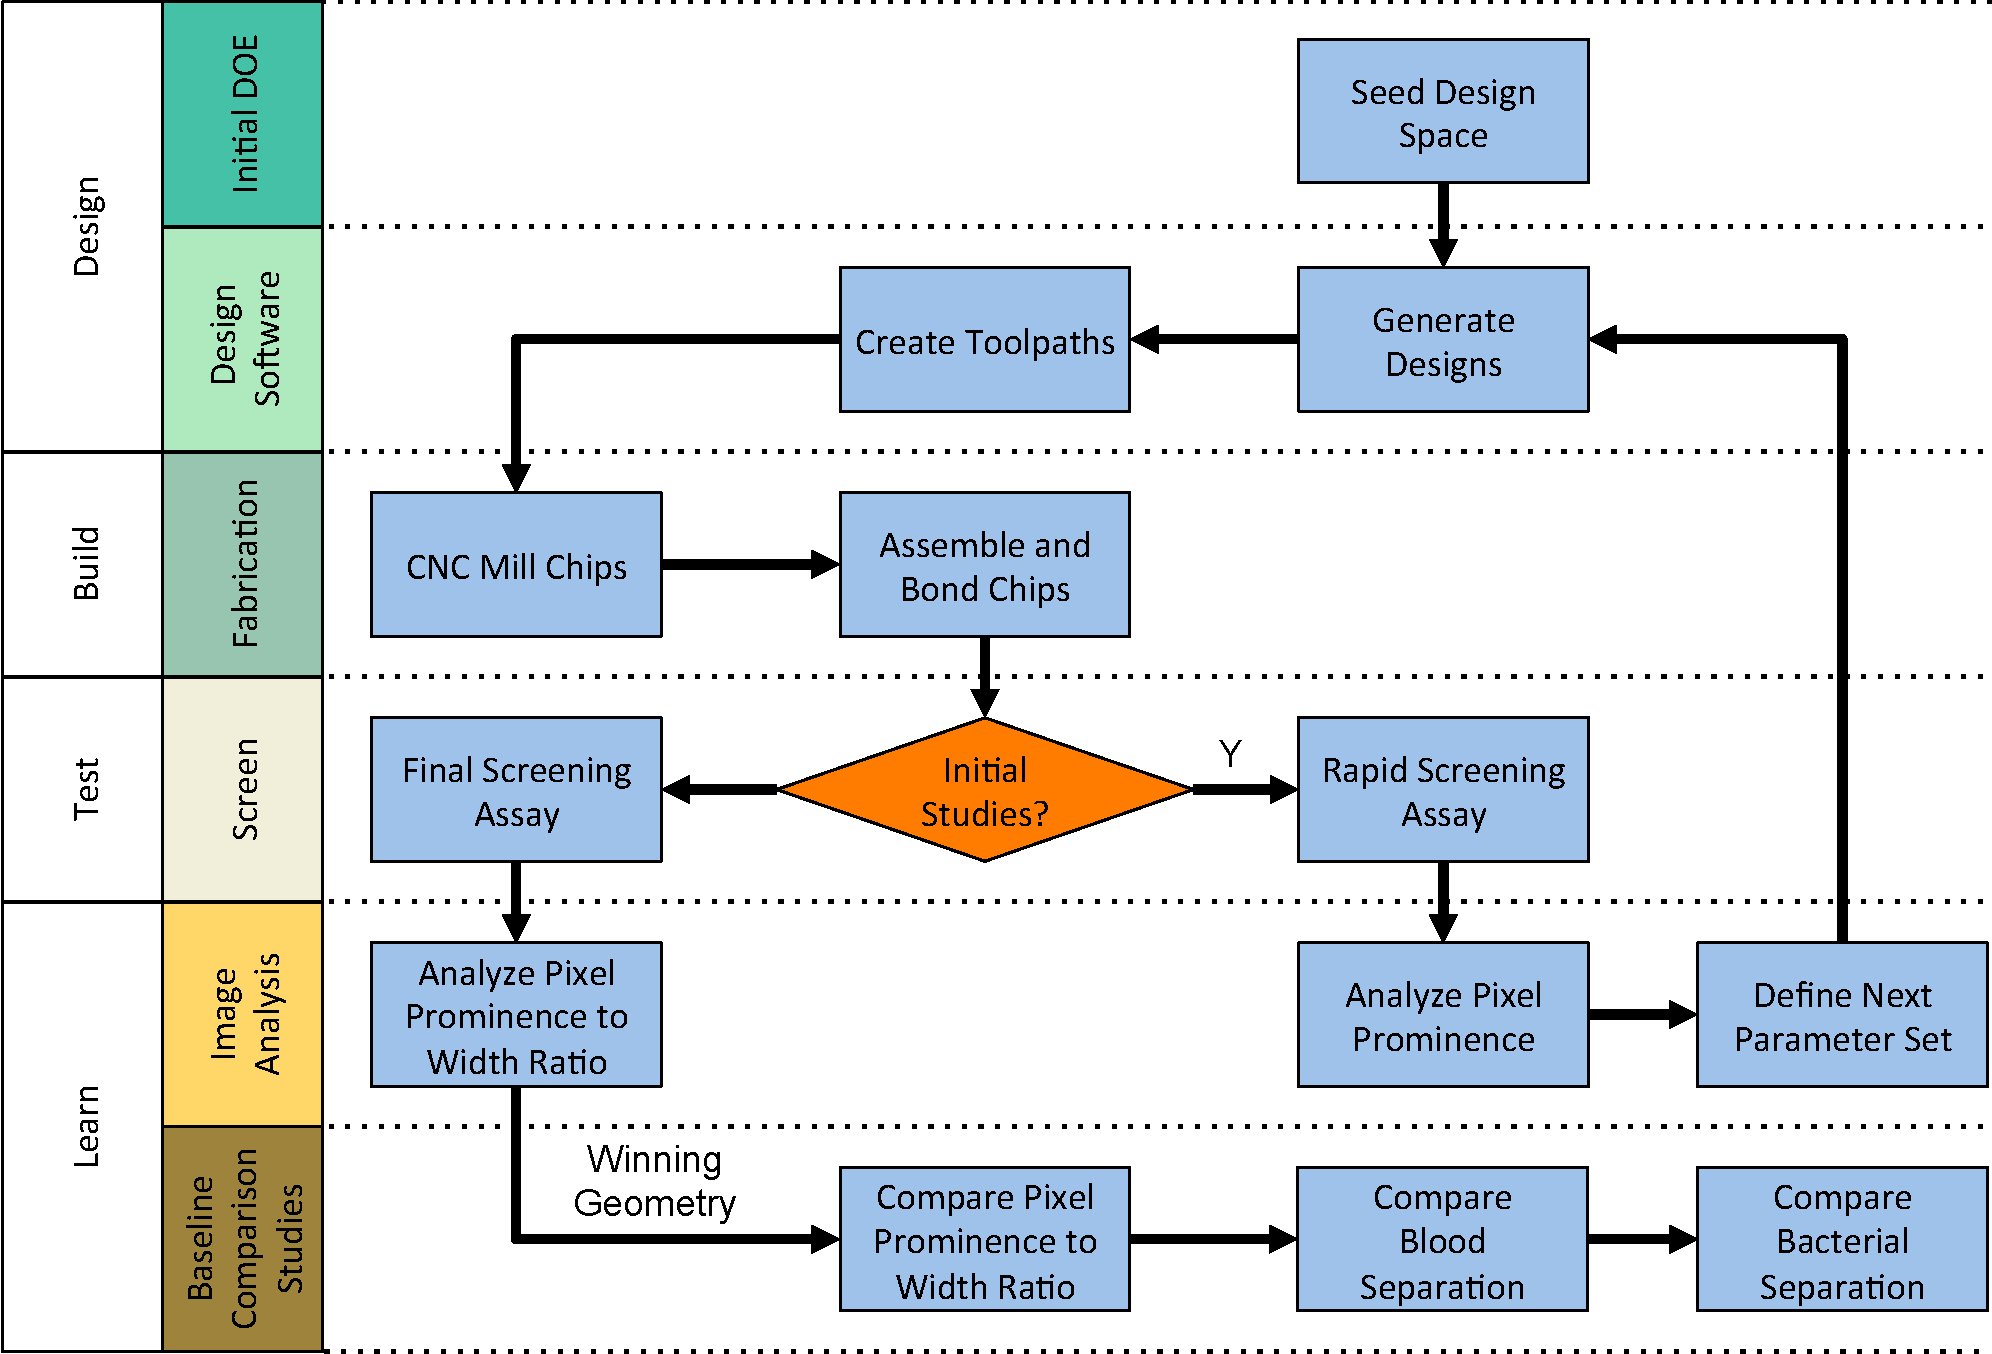
\includegraphics[width=14cm]{flow.pdf}
  %\end{minipage}\hfill
%\caption{Rapid Prototyping Workflow.}
%\label{fig:flow}       % Give a unique label
%\end{figure}


\begin{figure}[htb]
  \begin{minipage}[t]{0.99\linewidth}\centering
    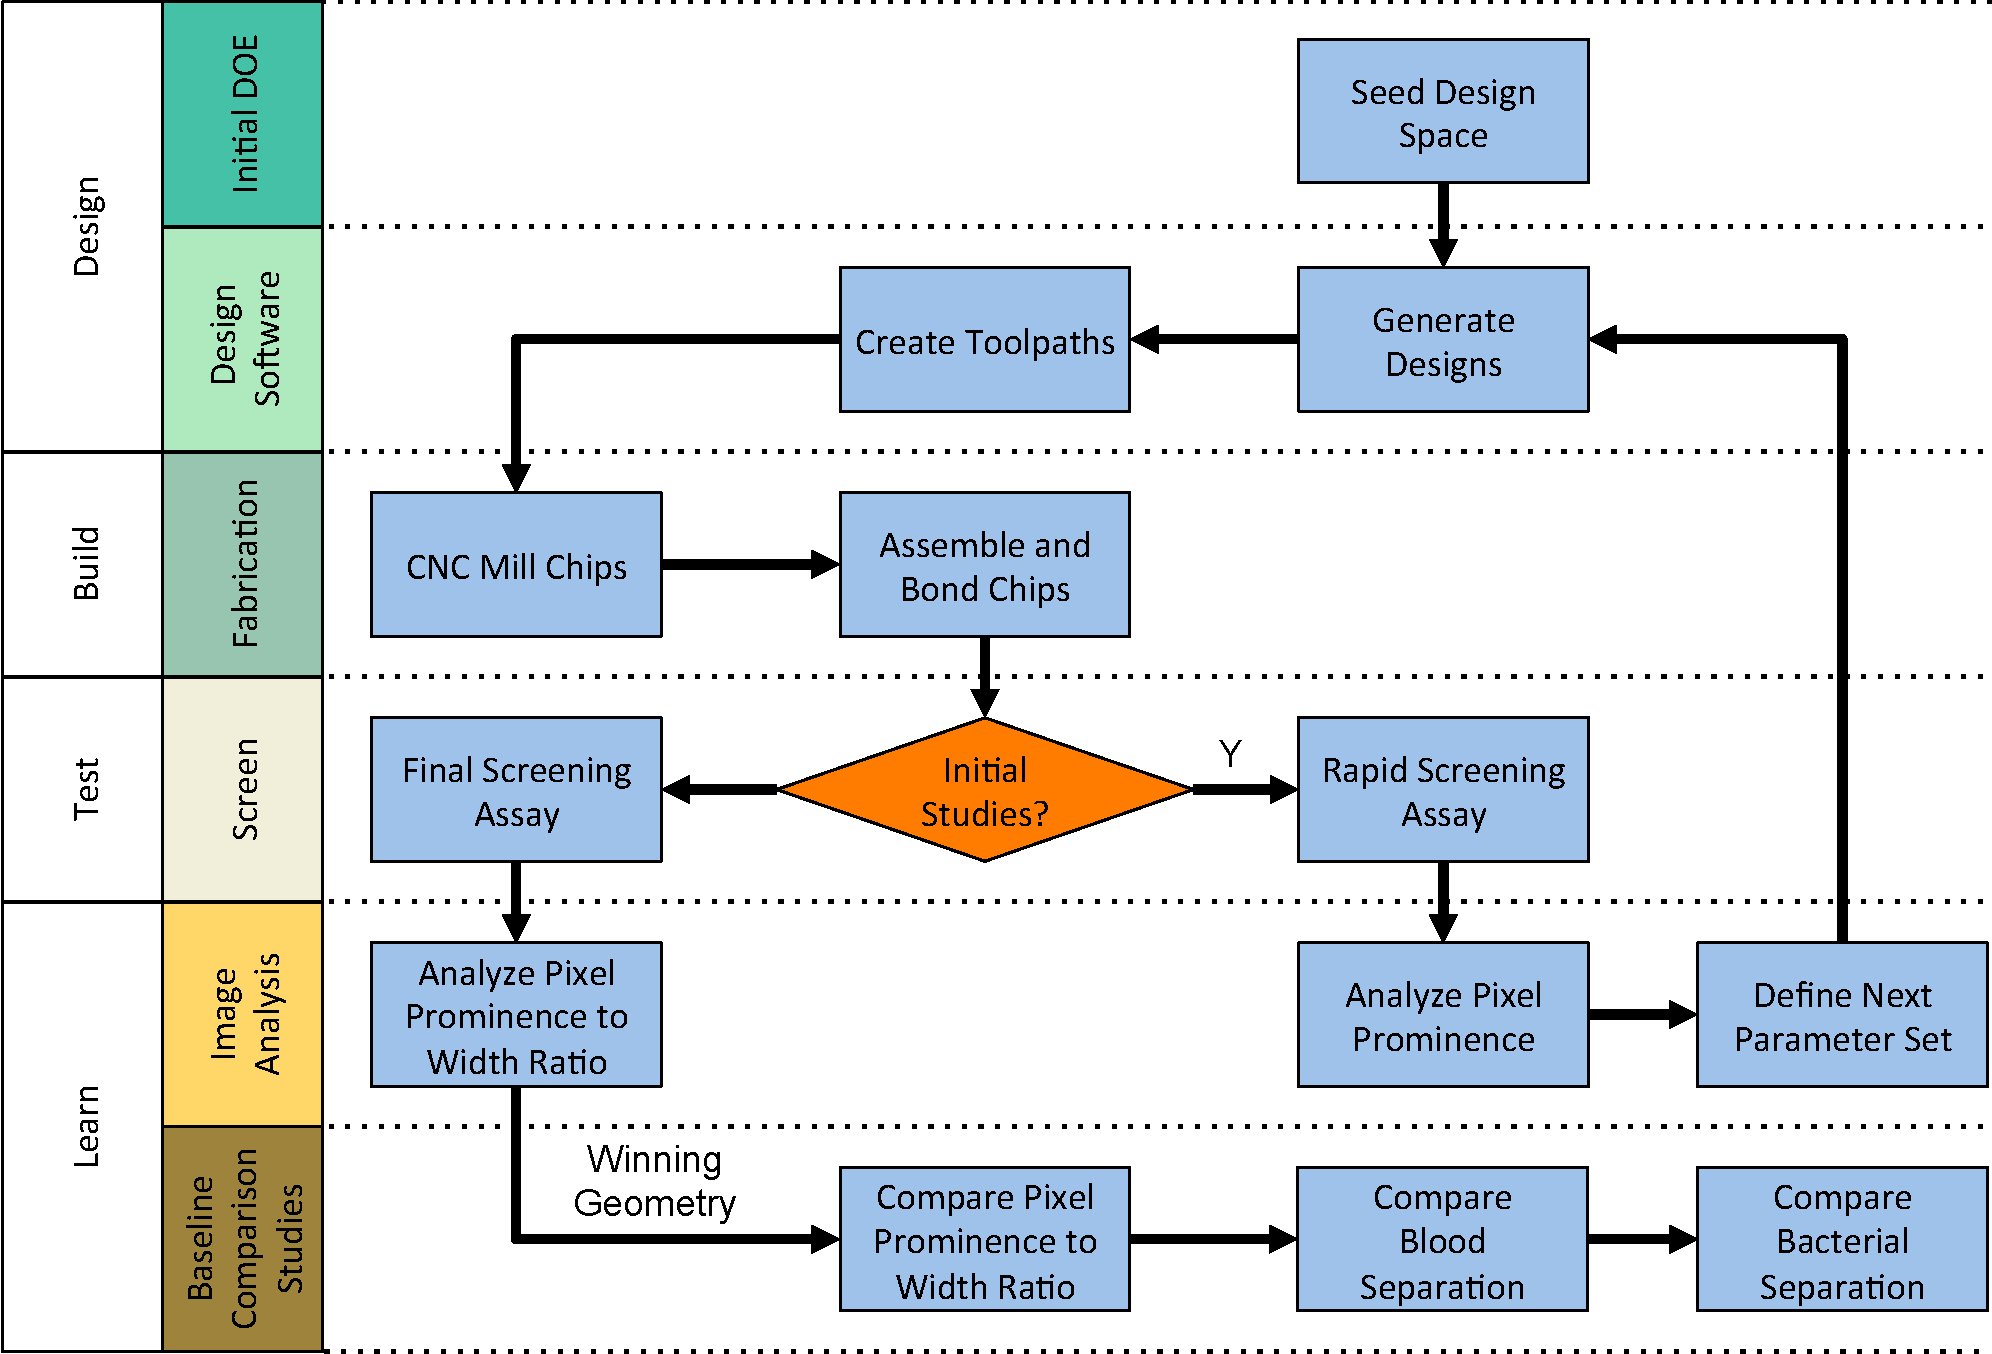
\includegraphics[width=14cm]{flow.pdf}
  \end{minipage}\hfill
  \caption[Rapid prototyping workflow]{Iterative rapid prototyping and testing workflow. The design space was first seeded using a design of experiments tool known as an orthogonal array, which minimizes the number of necessary experiments when compared to a full-factorial experimental analysis (Section \ref{ssec:seeding}). Trends were then identified within single geometric variables and experimentally explored. These variable isolation studies were repeated until a fully functional design set was achieved (Section \ref{ssec:iso}). The best performing device geometry emerging from the workflow, Chip 2.0, is then compared to the baseline using image processing, blood separation, and, finally, bacterial separation tests (Section \ref{ssec:comparison}).}
\label{fig:flow}       % Give a unique label
\end{figure}

Devices were screened in rapid succession using an image-based performance parameter of RBC acoustophoresis,  described in Section \ref{sec:img}, while varying two measures of merit: dissipated power and volumetric flow rate. As a final validation, the improved design was compared to the baseline in the task of separating bacteria from blood and shown to achieve comparable separation with significant advantages in the figures of merit. This improved device offers increased throughput and reduced power requirements and could improve performance in future point-of-care plastic acoustofluidic devices.

Figure \ref{fig:flow} illustrates the iterative workflow used in conducting the study, further described in Section \ref{sec:experiment}. Section \ref{sec:experiment} summarizes the approach used to design variable chip geometries and defines the two types of tests used in the screening phase of the workflow. Section \ref{sec:methods} outlines the methods used to screen separation performance from microscope images. Finally, Section \ref{sec:results} presents the results of the device screening as well as the winning design's performance when compared to that of the baseline geometry. 

\begin{figure}[htb]
  \begin{minipage}[t]{0.99\linewidth}\centering
    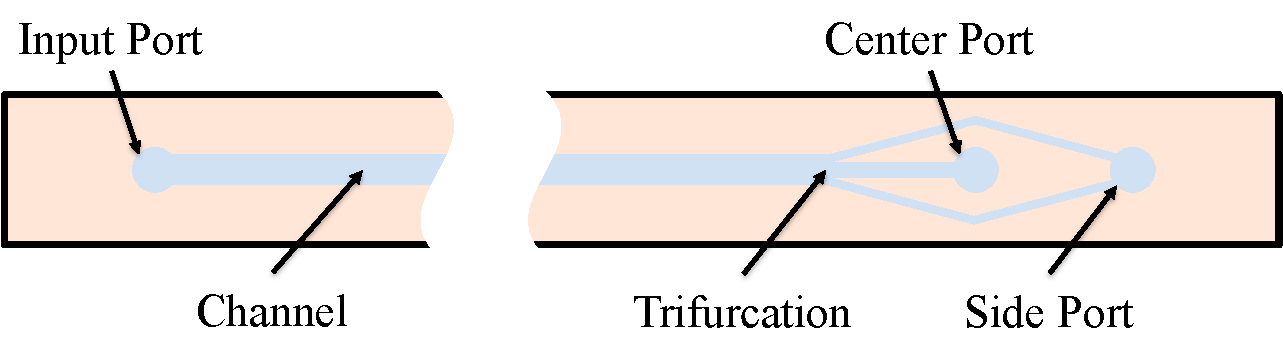
\includegraphics[width=14cm]{chip}
    \medskip
    \centerline{(a)}
  \end{minipage}\hfill\\
  \begin{minipage}[t]{0.99\linewidth}\centering
    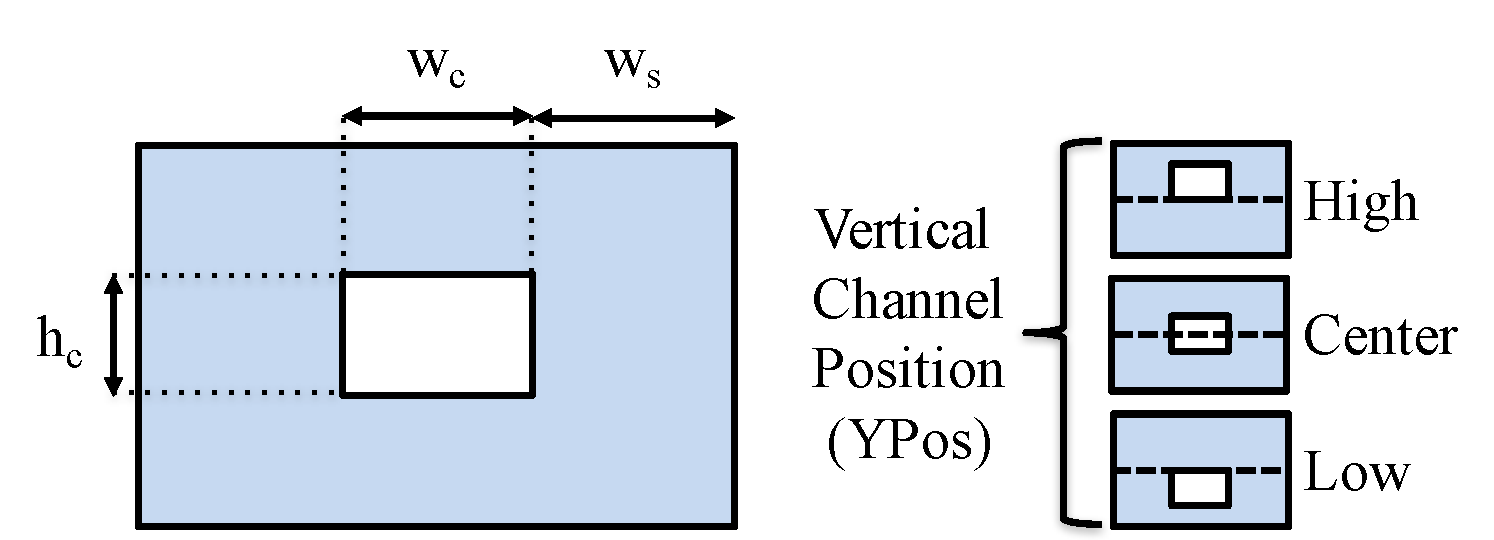
\includegraphics[width=14cm]{2D}
    \medskip
    \centerline{(b)}
  \end{minipage}
  \caption[Acoustofluidic separation device and 2D geometric definitions]{Acoustic separation device. (a) Complete trifurcated microfluidic separation chip. (b) Definitions for each two-dimensional geometry included in the study. Note that the definitions apply to the fluidic channel upstream of the trifurcation.} 
  \label{fig:geometry}
\end{figure}


Figure \ref{fig:geometry}a. is a top-down, two-dimensional drawing of the trifurcated acoustic separation device. The device functions by focusing large particles, such as RBCs and WBCs, to the center port, while smaller particles (e.g., platelets, bacteria, etc.) are collected at the side port. This trifurcated device is used in the blood and bacterial separation experiments. In order to reduce manufacturing complexity, devices screened using the methods outlined in Sections \ref{sssec:rapidScreen} and \ref{sssec:finalScreen} consist only of the input port; fluid channel, defined as the channel upstream of the trifurcation; and a single output port. The cross-sectional geometries, defined in Figure \ref{fig:geometry}b., apply to this simplified device design. 

\section{Experimental Methodology}
\label{sec:experiment}

\subsection{Rapid Prototyping}
\label{sec:rp}
This study relied upon the ability to design and fabricate iterations of chip geometries in a rapid process informed by experimental tests. The traditional workflow of conventional machining requires a fully specified mechanical drawing and changes to the design may demand regeneration of the solid model and revised setup of the milling instrument.  This section describes how these limitations were mitigated using free and open-source design software in conjunction with a \$3,199 USD desktop micromill (Othermill Pro, Other Machine Co., Berkeley, CA, USA).  Microchannels with parameterized dimensions were systematically fabricated with a minimum of operator intervention.

\begin{minipage}{0.95\linewidth}
\begin{lstlisting}[caption={The custom OpenSCAD library allows solid model creation using just a single line of code},label={lst:chip}, frame=single, language=scad]
  chip(Wc=0.55,Hc=0.25,Ws=0.85,YPos=high);
\end{lstlisting}
\end{minipage}

\begin{figure}[htb]
  \begin{minipage}[t]{0.99\linewidth}\centering
    
\includegraphics[width=14cm]{PaperExampleListing1}
  \end{minipage}\hfill
  \caption[Output single solid geometry]{Output solid geometry of Listing 1, including bonding plate.}
  \label{fig:listing1}
\end{figure}

\begin{minipage}{0.95\linewidth}
\begin{lstlisting}[caption={The single line of code in Listing \ref{lst:chip} can then be iterated upon to form an array of different device geometries that can be sent directly to a CAM tool for toolpath generation}, label={lst:chipLayout}, frame=single, language=scad]
include<chip.scad>

wc=[1.5,1,0.5];		 
ws=[0.5,1.5,2.5];
hc=[0.1,0.2,0.25];
ypos=[high,high,high];
Spacing=0.79375;         //End Mill Diameter

numChips=len(wc);	 //Total chips to make

module chipLayout(){
  //Iterate over number of chips
  for(i=[0:(numChips-1)]){
    let (ChipY=wc[i]+ws[i]*2){
      //Correctly space chips apart
      translate([0,2*i*(ChipY+Spacing),0])
      chip(Wc=wc[i],Hc=hc[i],Ws=ws[i],YPos=ypos[i]);
    }
  }
}
\end{lstlisting}
\end{minipage}


\begin{figure}[htb]
  \begin{minipage}[t]{0.99\linewidth}\centering
    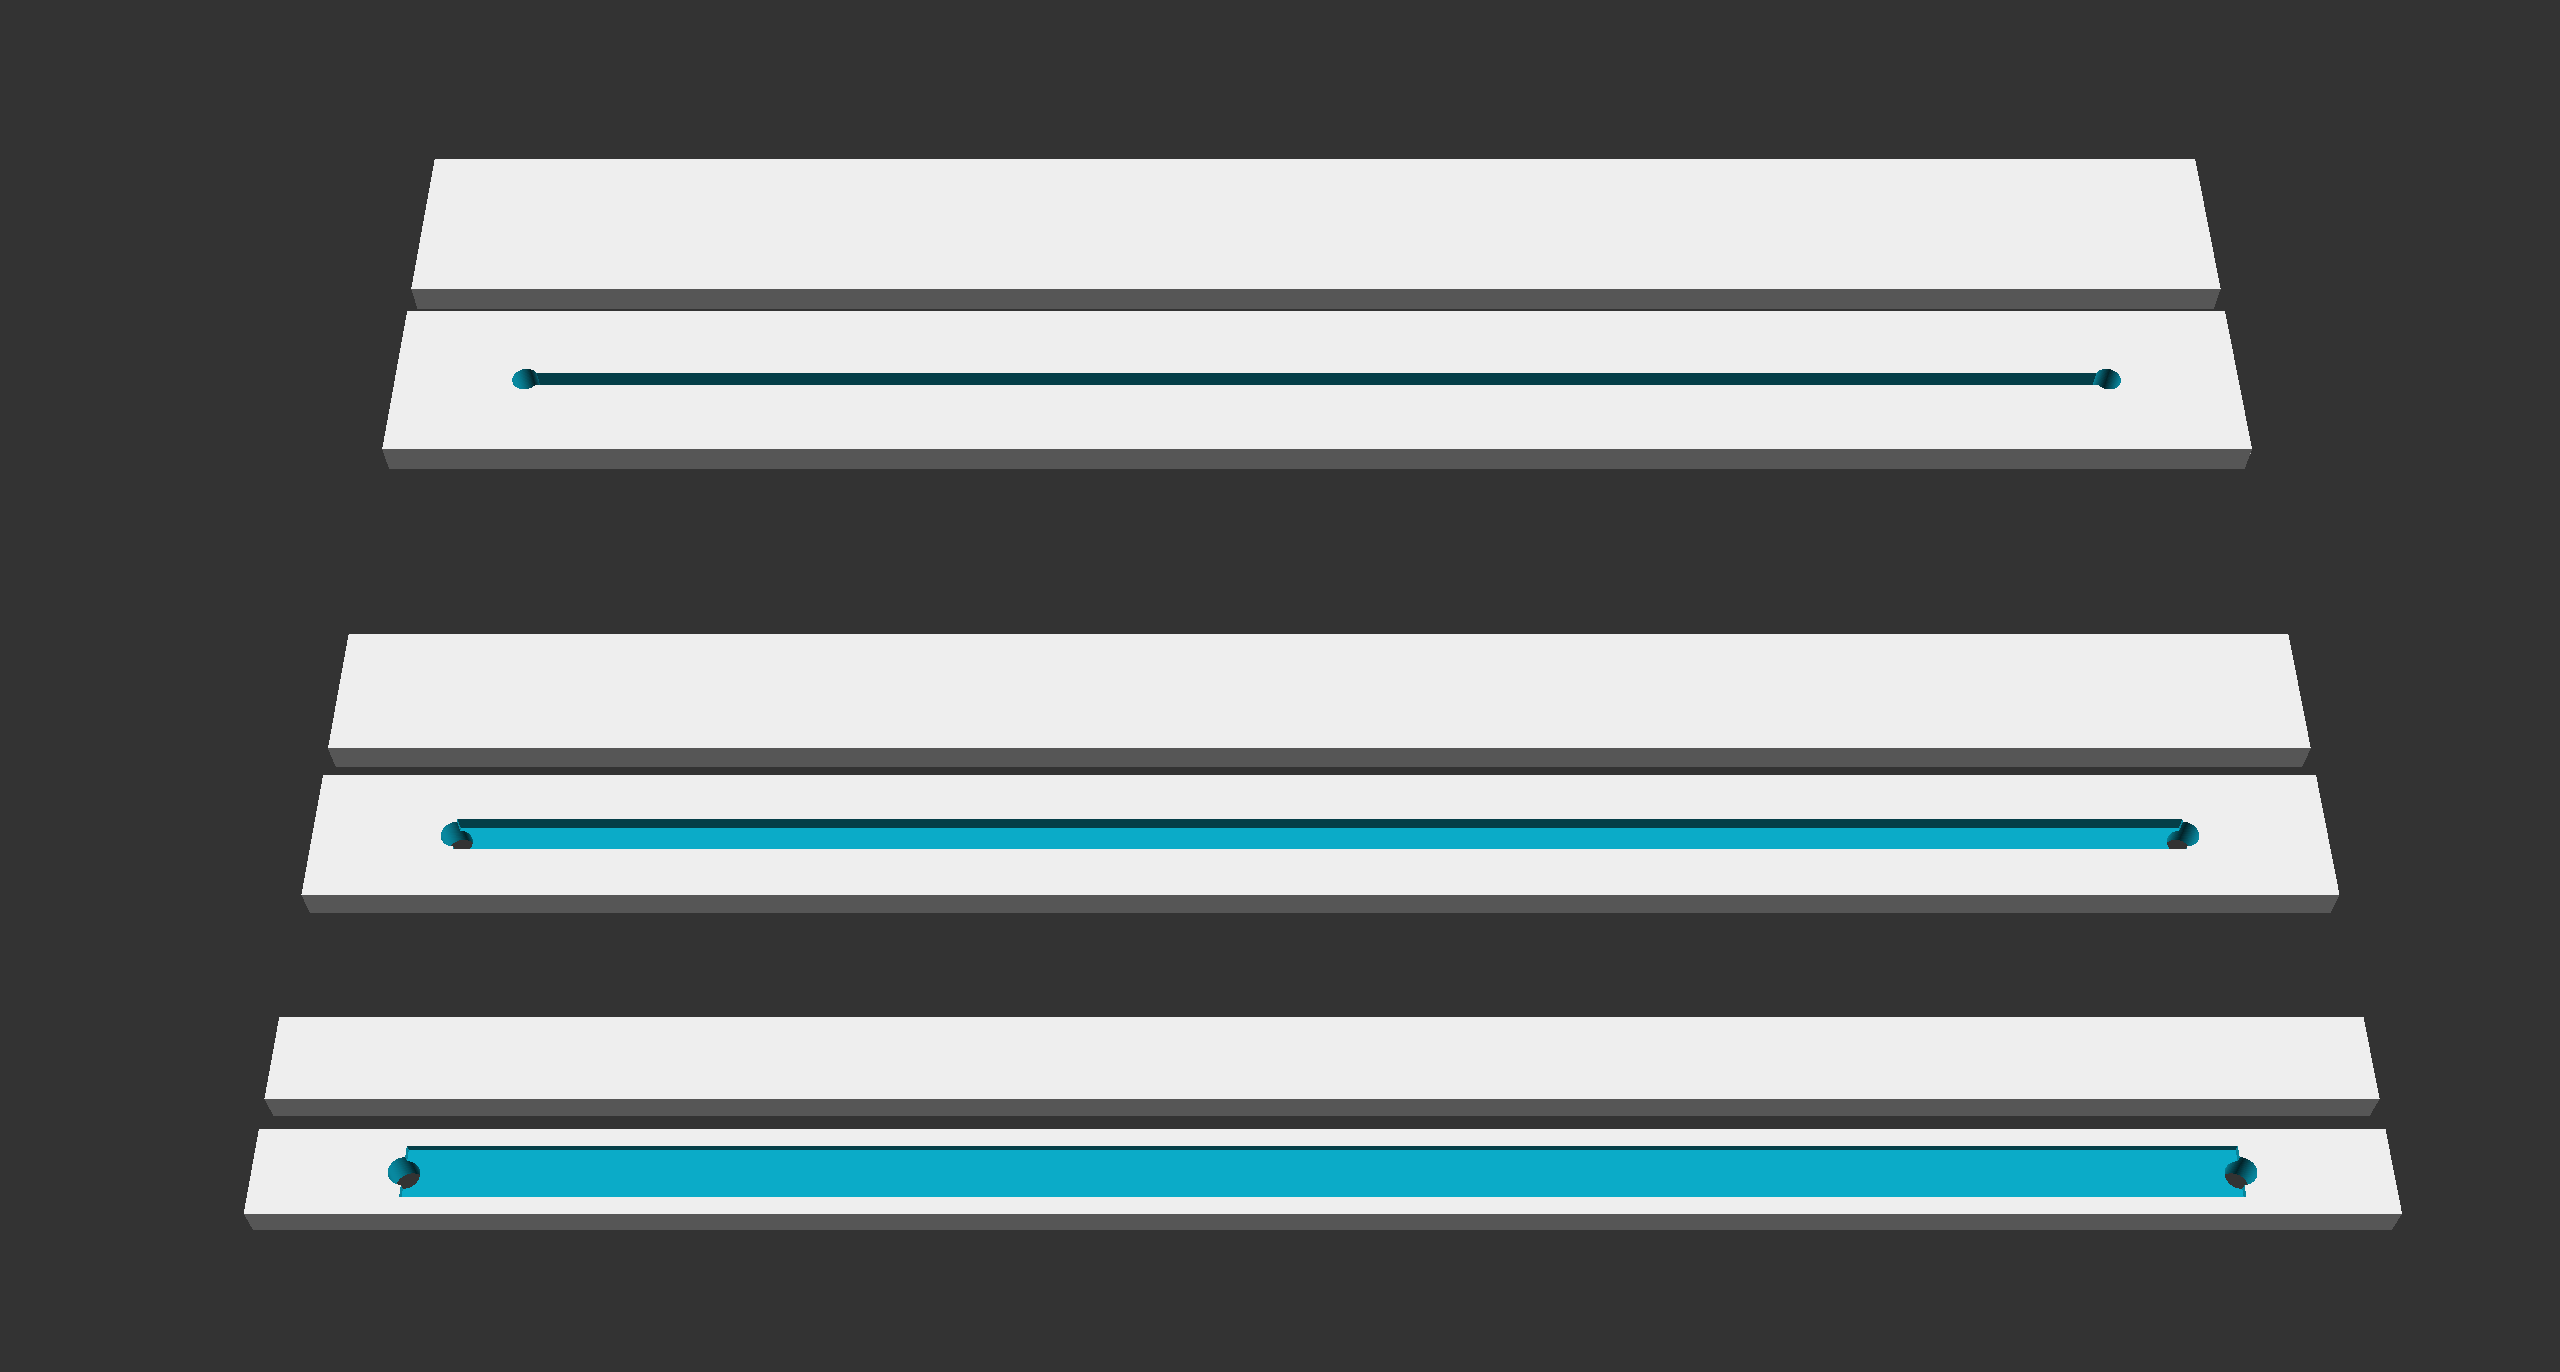
\includegraphics[width=14cm]{ExampleLayout}
  \end{minipage}\hfill
  \caption[Example layout of multiple device designs]{Output solid geometry of Listing 2, which includes three different designs and their corresponding bonding plates.}
	\label{fig:layout}
\end{figure}

\subsubsection{Design Generation}
\label{ssec:design}
Three levels of software are required to design and fabricate a novel chip geometry using a computer numerical control (CNC) micromill: a computer aided design (CAD) tool is used to create a solid model of the device; computer aided manufacturing (CAM) software generates the commands (also called toolpaths) that are sent directly to the micromill; and control software manages the connection between a computer and the micromill and sends individual toolpaths to the micromill. 

Device designs were created using OpenSCAD \cite{wikiOpenScad}, a free and open source CAD tool that reads script files to generate solid models. A custom library was used to create solid models using just the geometric parameters outlined in Figure \ref{fig:geometry}b. as inputs. Figure \ref{fig:layout} shows how an array of distinct solid models can be created from a few lines of code shown in Listing \ref{lst:chipLayout}. This array of designs is spaced according the size of the endmill used by the CNC to cut out each design, thus allowing for seamless processing by CAM software (Autodesk Fusion 360).

\subsubsection{Fabrication}
\label{ssec:fab}

Micromilling has demonstrated advantages for low-volume prototyping of plastic microfluidic devices in terms of time and cost when compared to other fabrication methods such as embossing and injection molding \cite{guckenberger2015micromilling}. While such studies claim that micromilling devices using an outside source can lower costs to \$137 per batch and 11-15 days of turn-around time, these costs only consider material costs and not labor, which can drive up the cost of prototyping an order of magnitude \cite{guckenberger2015micromilling}. Costs per device can be lowered to less than \$1 if devices can be fabricated in-house; however, the costs associated with establishing such capabilities can be prohibitive. It is only very recently that high quality micromills have been available at low cost: As recently as 2015, micromills capable of achieving resolutions at or below 25$\mu$m were available for a minimum of \$15k \cite{guckenberger2015micromilling}. The large footprints and noise associated with these machines made them inappropriate for use within a microfluidics laboratory. Additionally, the cost in terms of expertise required to operate a micromill is non-trivial. The software stack associated with generating toolpaths for a micromill does not currently resemble the simplicity of other CNC machines such as 3D printers. Traditional micromilling requires a suite of CAM tools that demand extensive knowledge of various tooling strategies such as feed rate, depth of cut and spindle speed that vary with each material and tool size. 

Recent advances in micromilling has led to the formation of a new class of desktop micromills, which can approach 25$\mu$m resolution at costs starting at \$2,500 all in a form-factor appropriate for a typical laboratory bench \cite{yen2016cost}. While these new machines still require knowledge of CAD and CAM software tools, research in automation techniques specifically for micromilling microfluidics is beginning to bear fruit \cite{silva2016iwbda}\cite{mcdaniel2017case}. This study leverages these advancements to quickly manufacture distinct acoustofluidic device designs at a negligible cost when compared to outsourcing fabrication.

\subsection{Device Evaluation}
\label{sec:eval}
We organized this study into four types of experiments: rapid screening, final screening, blood separation, and bacterial separation, progressing toward the selected design and then validating its performance in a series of functional tests. Rapid screening tests were conducted on two initial sets of designs for which the functionality of each design in the set could not be assumed, as shown in Figure \ref{fig:flow}. The methodology for this test is outlined in Section \ref{sssec:rapidScreen}. The results of these two initial rapid screening tests were then used to inform the parameter set of a final, more involved, screening test described in Section \ref{sssec:finalScreen}. Next, the winning geometry after final screening, hereafter referred to as Chip 2.0,  was compared to that of the baseline geometry in two different experiments measuring a device's ability to focus RBCs.  Finally, Chip 2.0 was compared to the baseline in experiments separating bacteria from diluted whole blood. The methodologies for each experiment are outlined in the subsections below. 

The screening tests analyzed microscope images and derived pixel intensities as an indicator of RBC focusing performance. This method assumes that higher concentrations of RBCs will appear visibly darker, and hence have a higher inverse grayscale value, when better acoustic focusing is present \cite{barnkob2012measuring}. Figures \ref{fig:pixelPerformance} and \ref{fig:microscopePics},  demonstrate that in conditions conducive to good focusing (e.g., lower flow rate and higher dissipated power) the observable band of blood cells will appear narrower and darker and thus have a correspondingly higher inverse grayscale value within this band. 

\begin{figure}[htb]
  \begin{minipage}[t]{0.49\linewidth}\centering
    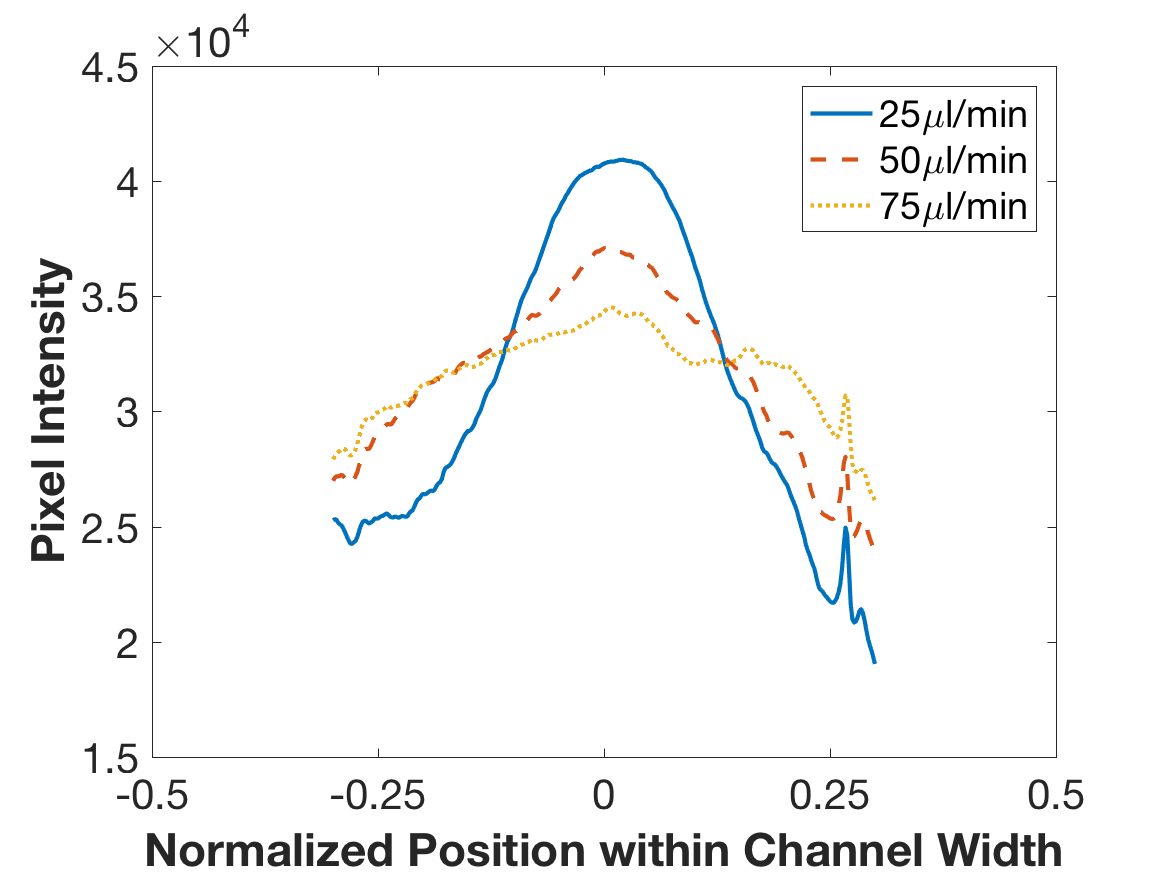
\includegraphics[width=7cm]{Baseline3PromFlow}
    \medskip
    \centerline{(a)}
  \end{minipage}\hfill
  \begin{minipage}[t]{0.49\linewidth}\centering
    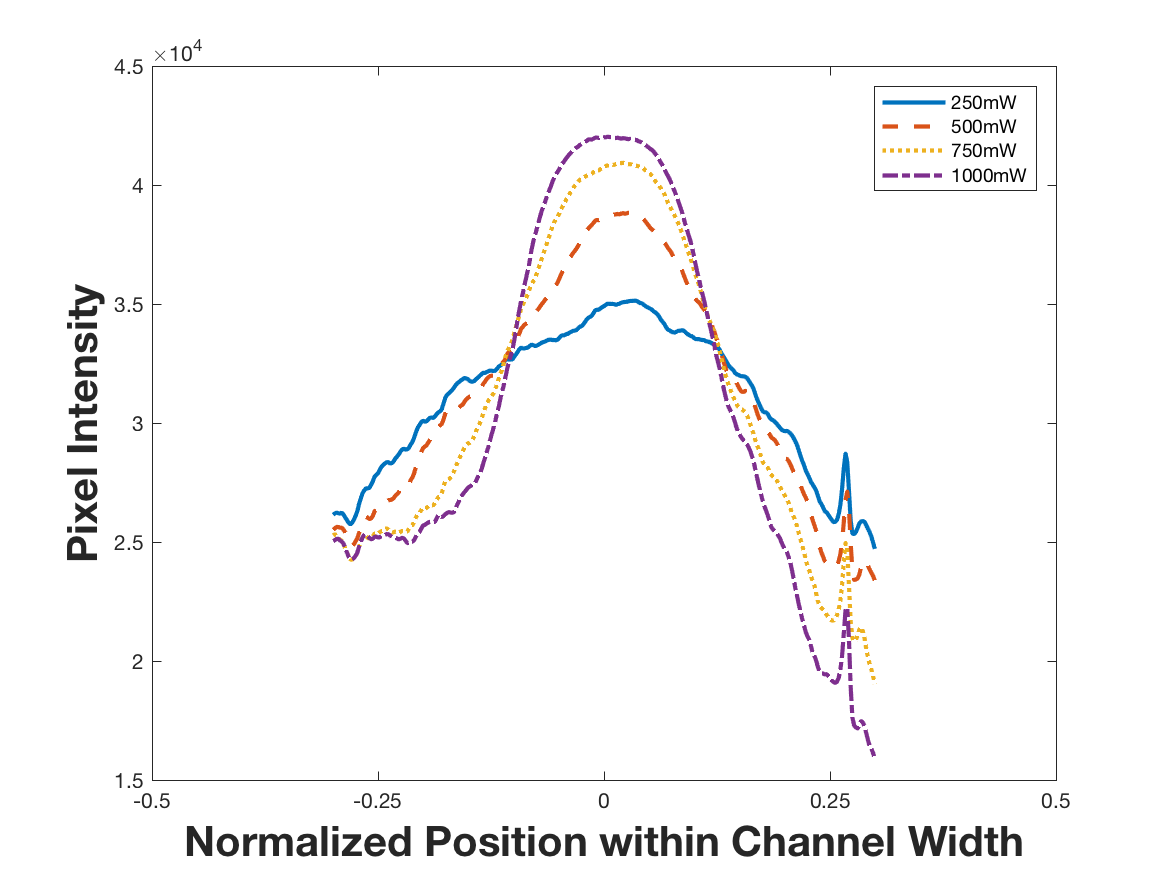
\includegraphics[width=7cm]{Baseline3PromPower}
    \medskip
    \centerline{(b)}
  \end{minipage}
  \caption[Pixel grayscale values across the width of the fluidic channel]{Pixel intensity as a surrogate for RBC focusing performance. Inverted pixel grayscale values (i.e., darker areas have a higher value) across the width of the fluidic channel. (a) Power is held constant at 750 mW while flow rate is varied. Note that maximum pixel intensity, and thus focusing performance, increases as flow rate is decreased. (b) Flow rate is held constant at 25 $\mu$l/min, while power is varied. Note that focusing performance increases as power is increased.}
	\label{fig:pixelPerformance}
\end{figure}

\begin{figure}[htb]
  \begin{minipage}[t]{0.49\linewidth}\centering
    
\includegraphics[width=7cm]{25ul250mWBaseline_3}
    \medskip
    \centerline{(a) 250mW}
  \end{minipage}\hfill
  \begin{minipage}[t]{0.49\linewidth}\centering
    
\includegraphics[width=7cm]{25ul500mWBaseline_3}
    \medskip
    \centerline{(b) 500mW}
  \end{minipage}\\
  \begin{minipage}[t]{0.49\linewidth}\centering
    
\includegraphics[width=7cm]{25ul750mWBaseline_3}
    \medskip
    \centerline{(c) 750mW}
  \end{minipage}\hfill
  \begin{minipage}[t]{0.49\linewidth}\centering
    
\includegraphics[width=7cm]{25ul1000mWBaseline_3}
    \medskip
    \centerline{(d) 1000mW}
  \end{minipage}\\
  \caption[Microscope images at resonant frequency for increasing power levels]{Microscope images of focusing performance at resonant frequency with increasing power at levels of 250mW (a), 500mW (b), 750mW (c), 1000mW (d). The plots in Figure \ref{fig:pixelPerformance}(b) are derived directly from these images.}
	\label{fig:microscopePics}
\end{figure}

The two types of screening tests, rapid screening and final screening, each have different assumptions regarding the nature of their input parameter sets. In the rapid screening test a device may not exhibit acoustic focusing at any frequency under the experimental conditions; thus, the performance parameter determines the existence of acoustic focusing, but does not discern the relative quality of focusing between devices.  In contrast, the final screening test attempts to compare the relative performance of devices that exhibit some acceptable measure of focusing performance. 

The latter separation experiments measured a device's ability to maintain cell separation performance while minimizing dissipated power to the transducer (i.e. amplitude of acoustic excitation) and maximizing sample throughput (i.e., volumetric flow rate). Maximizing the volumetric flow rate will enable the largest volume of input sample to be enriched in the shortest amount of time. Minimizing the power requirements of the system is another important measure of merit because heat generated in the transducer and in the PS channel during actuation may lead to delamination of the channel or may be harmful to the clinical sample. Therefore, it is best to drive the system at the smallest amplitude necessary to achieve acceptable performance. 

\subsubsection{Rapid Screening Test}
\label{sssec:rapidScreen}

The purpose of the rapid screening test was to discover functional device designs, i.e., designs that could focus blood, and the frequencies at which they operate. Functionality of an acoustofluidic device was determined by analyzing the strength of focusing bands whose maxima occurs within the center fifth of the channel width, as the purpose of the device is to focus RBCs into the center channel of the trifurcation shown in Figure \ref{fig:geometry}. Thus, in order to affirm the decision node labeled ``Focusing Observed Across Set'' in Figure \ref{fig:flow}, the point of maximum pixel intensity must be present in the center fifth of the channel for the device under test. 

Each set of devices was tested under the same power and flow conditions while sweeping through a frequency band  of  0.50 -- 2.00 MHz.  This range was informed by the optimum frequency of the baseline device (1.012 MHz).  The transducer was selected with a resonant frequency of 2.34 MHz to avoid confounding effects of transducer resonance. The flow rate was set such that the average velocity in each chip was  1.94 cm/sec, a value that is equivalent to 100 $\mu$l/min in the baseline device. The input power to the RF amplifier was set such that the average dissipated power at the transducer was 1 W at 1 MHz. Electrical equipment settings (e.g., input voltage, RF amplifier gain, etc.) for this condition (i.e., 1 W at 1 MHz) were held constant as the frequency was varied. Within the tested bandwidth photos of the downstream end of the channel were taken in 10 kHz increments, from which a number corresponding to the maximum peak prominence was returned.   Prominence is a measure of a ``peak'' in pixel intensity and is defined further in the Methods section. The maximum peak prominence for the entire frequency band constituted the score for that particular design. An example frequency sweep is shown in Figure \ref{fig:freqSweep}.

%(\textbf{FOR JASON:} $Q=VA$; $A=0.043cm*0.02cm=0.00086cm^2$; $Q=100\mu L/min=0.1cm^3/min$; $V=\frac{Q}{A}=\frac{0.1}{0.00086}=116.3 cm/min=1.94 cm/sec$)

\begin{figure}[htb]
  \begin{minipage}[t]{0.99\linewidth}\centering
	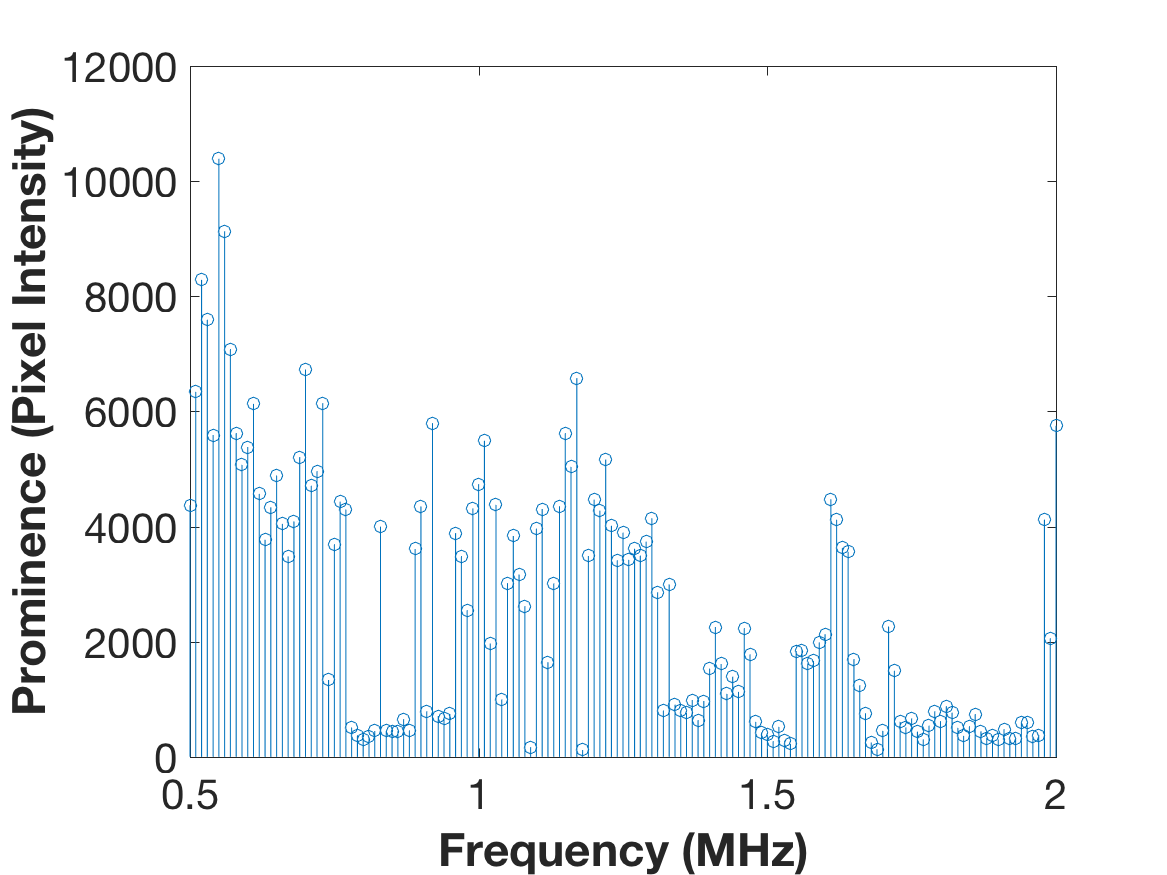
\includegraphics[width=12cm]{freqSweep}
  \end{minipage}\hfill
	\caption[Prominence versus frequency across swept bandwidth]{Prominence versus Frequency for a fixed input voltage for device 4L9 in Table \ref{tab:geometries}. Images were captured in 10 kHz increments over the bandwith extending from 0.5 MHz to 2 MHz, inclusive.}
	\label{fig:freqSweep}
\end{figure}

\subsubsection{Final Screening Test}
\label{sssec:finalScreen}

The final screening test served to discriminate between devices that exhibited RBC focusing on the rapid screening test. This was accomplished by manually tuning the device to its optimum frequency (by visual inspection of the RBC focusing) and then modulating the measures of merit. Three flow rates (25 $\mu$l/min, 50 $\mu$l/min, and 75 $\mu$l/min) and four power levels (250 mW, 500 mW, 750 mW, and 1000 mW) were studied. A microscope image was captured for each combination of flow rate and power level, from which the ratio of peak prominence to width was calculated in accordance with the method described in Section \ref{ssec:promToWidth}.  The ratio of peak prominence to width serves as a predictor of the device's ability to separate RBCs.

\subsubsection{Blood Separation Test}
\label{ssec:bloodAssay}

The purpose of the blood separation test is to measure a device's ability to focus RBCs to the center port of the device at a series of combinations of flow rate and power settings. A test of this sort has proven useful in assessing or comparing the acoustic energy density in several device configurations for applications ranging from high-throughput cell sorting \cite{adams2012high}\cite{mueller2013continuous} to plasmapheresis \cite{lenshof2009acoustic}. Samples of dilute whole blood were collected from both side and center ports for each setting according to the protocol established in Section \ref{sec:sampleMeasurement}. Performance is measured using RBC separation percentage, calculated by dividing the number of RBCs collected from the center port and dividing by the total number of RBCs collected from both outlet ports.

\subsubsection{Bacterial Separation Test}
\label{ssec:bacteriaAssay}

The goal of the bacterial separation experiments is to determine the maximum capacity of a chip design in its ability to separate bacteria from blood, as has been demonstrated in other acoustic microfluidic devices \cite{ohlsson2016integrated}\cite{li2016acoustofluidic}. The operational capacity of a chip is evaluated in terms of the two measures of merit: volumetric flow rate and average dissipated power, each tested with the other fixed.  Bacterial separation is measured at the point of minimum power or maximum flow rate required to achieve 90\% separation of RBCs, measured by the ratio of colony forming units (CFU) to RBCs present in the side port.  Where power was varied, flow rate was held at 50 $\mu$l/min.  Where flow rate was varied, power was held at 1 W. 

\section{Methods}
\label{sec:methods}

\subsection{Materials and Assembly}
Polystyrene (PS) was selected as an appropriate material based on its relatively low attenuation and high acoustic impedance relative to other plastics \cite{mueller2013continuous}\cite{selfridge1985approximate}. The chip was sealed using a thermal bonding method previously described \cite{mueller2013continuous}. 0.75'' lengths of polyetheretherketone (PEEK) tubing served as an interface between the PS chip and the longer lengths of polyvinyl chloride (PVC) tubing used to introduce and collect sample. The rigid PEEK tubing was inserted into machined port cavities and affixed to the chip using epoxy (Epoxy 907, Miller-Stephenson, Danbury, CT, USA). 

Lengths of vinyl capillary tubing  were appended to the outlet ports to divide outlet volumes at a ratio of 60\% volume measured at the side port to 40\% at the center, using relative resistances. 

%tubing length was cut to match the ratio of hydraulic diameters of each channel. Once flow fractions matched outlet dimensions, the channel was primed with deionized (DI) water, followed by the sample.  Once the sample being tested occupied the total volume of the microfluidic chip and inlet/outlet tubing, the flow rate was set to appropriate setting on the syringe pump.  Control measurements were taken for each flow rate with the acoustics off to validate flow fraction as well as cellular behavior within microfluidic chip.  Samples were collected in conical tubes and measured for flow fraction and cell quantity calculations. The resonant frequency was found visually by observing the focusing stream -- the most compact stream reveals the resonant frequency.  Once the resonant frequency was found, powers were swept by increasing RF amplifier gain to encompass the experimental parameters.  For each sample, weights and hematology data was taken and entered into a database.  MATLAB was used for further data analysis and plotting.  

The sealed chip was mounted to a lead zirconate titanate (PZT) transducer (APC International, PZT 850) with a published resonance of 2.34 MHz using low viscosity cyanoacrylate adhesive.  

\subsection{Image Processing and Analysis}
\label{sec:img}
Image processing software (ImageJ \cite{imagej}) was used to measure pixel intensities across the width of the channel, $W_c$, from which prominence was calculated. The prominence of the focused stream, as described in detail in Section \ref{ssec:prom} below, served as a measure of the degree of focusing and the performance of the chip. Prominence has advantages over raw pixel intensity for the purposes of comparison due to its self-normalizing nature. Since prominence is measured relative to points on the signal itself it is robust against irregularities inherent to the signal. These irregularities can take the form of variable lighting conditions between experimental runs, such as variations in environmental lighting, and illumination variabilities within a single microscope image's region of interest, such as skewed background intensities caused by shadows. 

%Peak prominence is used as a direct measure of merit for device rapid screening studies.  When a device is determined to function well based on its prominence score it is compared to the baseline geometry (final screening) using the ratio of peak prominence to half-prominence width, $\chi$ (Figure \ref{fig:algProg}c.). $\chi$ cannot be used during device screening as the metric can skew results by rewarding peaks with relatively small prominence values and correspondingly small widths. However, this metric is useful for comparing the quality of the most prominent peaks among different, commensurate, devices such as the winner of a design screening iteration and the baseline geometry.


\subsubsection{Definition of Prominence}
\label{ssec:prom}
Suppose an ordered signal is defined as in Equation \ref{eqn:sig}, where set $D$ consists of $N$ data points. Prominence is calculated by first finding all local maxima within the response set $D$ and then determining a reference point on the signal associated with each local maxima \cite{freeman1977corner}\cite{arge2013algorithms}. Briefly, this reference point is established by drawing a horizontal line in both the positive and negative directions from the local maxima (labeled as ``Scan High'' and ``Scan Low'', respectively, in Figure \ref{fig:algProg}) until either the end of the signal is reached (as in the case of $i_{high}$, in Figure \ref{fig:algProg}) or until the line intersects the signal itself ($i_{low}$, in Figure \ref{fig:algProg}), thus creating two sets of data points in the positive and negative directions. Minima are determined for each of the data sets, and prominence is then defined as the height of the local maxima relative to the maximum of these two established minima ($s_{ref}$). 

\begin{equation}
  \label{eqn:sig}
  \hfill s[n]=D \quad n=0,1,2,\cdots,N-1 \hfill
\end{equation}

A framework for defining prominence in a more formal terms begins by establishing the data structure for the signal of interest. Individual values are accessed by index such that $s[i]=d_i, d_i\in D$. Two discrete points $d_i \in D$ and $d_{i'} \in D$ are said to be $neighbors$ if $|i-i'| = 1$. A local maxima, hereafter called a $peak$, is a point $p$ where $d_i$ is greater than all of its neighbors, as defined in Algorithm \ref{alg:peaks}. The set of peaks $P \subset D$ consists of individual peak values $p \in P$. A peak is referenced by its index value $i$ in $D$ and the raw peak height is calculated by finding $s[i]$. The index in $D$ of peak $p$ is returned by the function $x(p)$. The height of peak $p$ is returned by the function $s[x(p)]$. Thus if $p \leftarrow d_i$, $x(p)=i$ and $s[x(p)]=d_i$. Prominence is then determined via Algorithm \ref{alg:prom}. 

%\paragraph{Paragraph headings} Use paragraph headings as needed.
%\begin{equation}
%a^2+b^2=c^2
%\end{equation}

\begin{figure}
\begin{algorithm}[H]
\DontPrintSemicolon
\SetKwFunction{AppendToP}{AppendToP}
\SetKwData{neighbors}{neighbors}
\KwData{Ordered data set $D$}
\KwResult{A list of peaks $P\subset D$}
\Begin{
$P \longleftarrow \emptyset$\;
\For{$d_i \in D$}{
    Find all $neighbors$ for $d_i \mid |i-i'|=1$
    $\AppendToP(neighbors)$
}
}
\caption{Find Peaks. Finds all local maxima in $D$ and returns them as a list of peaks $P$ as shown in Figure \ref{fig:algProg}(a). \label{alg:peaks}}
\end{algorithm}
\end{figure}

\begin{figure}
\begin{algorithm}[H]
\DontPrintSemicolon
\SetKwData{s_{low}}{s_{low}}
\SetKwFunction{AppendToWidth}{AppendToWidth}
\KwData{Ordered data set $D$ and a list of local maxima $P\subset D$}
\KwResult{A list of prominence values, $Prom$, for each local maxima, $p$}
\Begin{
$Prom \longleftarrow \emptyset$\;
  \For{$p_j \in P$}{
	\tcc{Scan Low}
	\For{$i = 0$ to $x(p_j)$}{
	  \If{$x(p_j)=0$}{
	    $i_{low}=x(p_j)$\;
	    Exit Loop\;
	  }
	  \ElseIf{$s[x(p_j)-i] \geq s[x(p_j)] \lor x(p_j)-i=0$}{
	    $i_{low}=x(p_j)-i$\;
	    Exit Loop\;
	  }
	}
	\For{$i = 0$ to $N-1$}{
	  \If{$x(p_j)=N-1$}{
	    $i_{high}=x(p_j)$\;
	    Exit Loop\;
	  }
	  \ElseIf{$s[x(p_j)+i] \geq s[x(p_j)] \lor x(p_j)+i=N-1$}{
	    $i_{high}=x(p_j)+i$\;
	    Exit Loop\;
	  }
	}
  $s_{low}=min(s[i_{low}] \to s[x(p_j)])$\;
  $s_{high}=min(s[x(p_j)] \to s[i_{high}])$\;
  $s_{ref}=max(s_{low},s_{high})$\;
  $Prom_j = s[x(p_j)] - s_{ref}$\;
  $\AppendToWidth(Prom_j)$\;
  }
}
\caption{\label{alg:prom}Calculate Prominence. Draw a horizontal line to the left (low) and right (high) of the peak until the end of the signal is reached or until the signal is intersected. Record the indices of each as $i_{low}$ and $i_{high}$, respectively. Find the minima in each set and use the maximum of the minima to set the reference level. Calculate a peak's prominence by subtracting the reference level from the raw signal value of the peak (Figure \ref{fig:algProg}(b-c))}
\end{algorithm}
\end{figure}

\subsection{Definition of Prominence to Width Ratio, $\chi$}
\label{ssec:promToWidth}
The half-prominence width of a peak of prominence $Prom$ is calculated by drawing two horizontal lines extending in the negative and positive directions from the point of half-prominence. These lines extend in either direction until either the end of the signal is reached or the line intersects the signal itself. The indices of these events in the negative and positive directions are recorded as $i^-$ and $i^+$, respectively. The peak width $HalfPromWidth$ is then defined as $|i^+-i^-|$, as described in Algorithm \ref{alg:width}. We reason that for equivalent separation performance, assuming a fixed ratio of flow to side and center ports \cite{ley2016continuum}, that the prominence half width scales with the channel width, therefore it is appropriate to normalize the peak width by the width of the channel. The final equation for $\chi$ is shown in Equation \ref{eqn:ratio}

\begin{figure}
\begin{algorithm}[H]
\DontPrintSemicolon
\SetKwData{s_{low}}{s_{low}}
\SetKwFunction{FindPeaks}{FindPeaks}
\KwData{A list of prominence values, $Prom$, for each local maxima, $p$}
\KwResult{A list of half-prominence peak widths $HalfPromWidth$, for each local maxima, $p$}
\Begin{
$Prom \longleftarrow \emptyset$\;
  \For{$p_k \in P$}{
	\tcc{Scan Left}
	\For{$i = 0$ to $x(p_k)$}{
	  \If{$x(p_k)=0$}{
	    $i^-=x(p_k)$\;
	    Exit Loop\;
	  }
	  \ElseIf{$s[x(p_k)-i] \leq s[x(p_k)]-\frac{Prom_k}{2} \lor x(p_k)-i=0$}{
	    $i^-=x(p_k)-i$\;
	    Exit Loop\;
	  }
	}
	\tcc{Scan Right}
	\For{$i = 0$ to $N-1$}{
	  \If{$x(p_k)=N-1$}{
	    $i^+=x(p_k)$\;
	    Exit Loop\;
	  }
	  \ElseIf{$s[x(p_k)+i] \leq s[x(p_k)]-\frac{Prom_k}{2} \lor x(p_k)+i=N-1$}{
	    $i^+=x(p_k)+i$\;
	    Exit Loop\;
	  }
	}
  $HalfPromWidth_k = i^+-i^-$\;
  $\AppendToWidth(HalfPromWidth_k)$\;
  }
}
\caption{\label{alg:width}Calculate Peak Width at Half Prominence. Draw a horizontal line to the left (-) and right (+) at the median of the prominence line until either the end of the signal is reached or until the signal is intersected. Record the indices of each as $i^{-}$ and $i^{+}$, respectively. The absolute value of the difference between these index values is the peak width at half prominence. \ref{fig:algProg}(d))}
\end{algorithm}
\end{figure}

\begin{equation}
\label{eqn:ratio}
\hfill \chi=Prom*\frac{W_c}{HalfPromWidth}\hfill
\end{equation}


\begin{figure}[htb]
  \begin{minipage}[t]{0.99\linewidth}\centering
	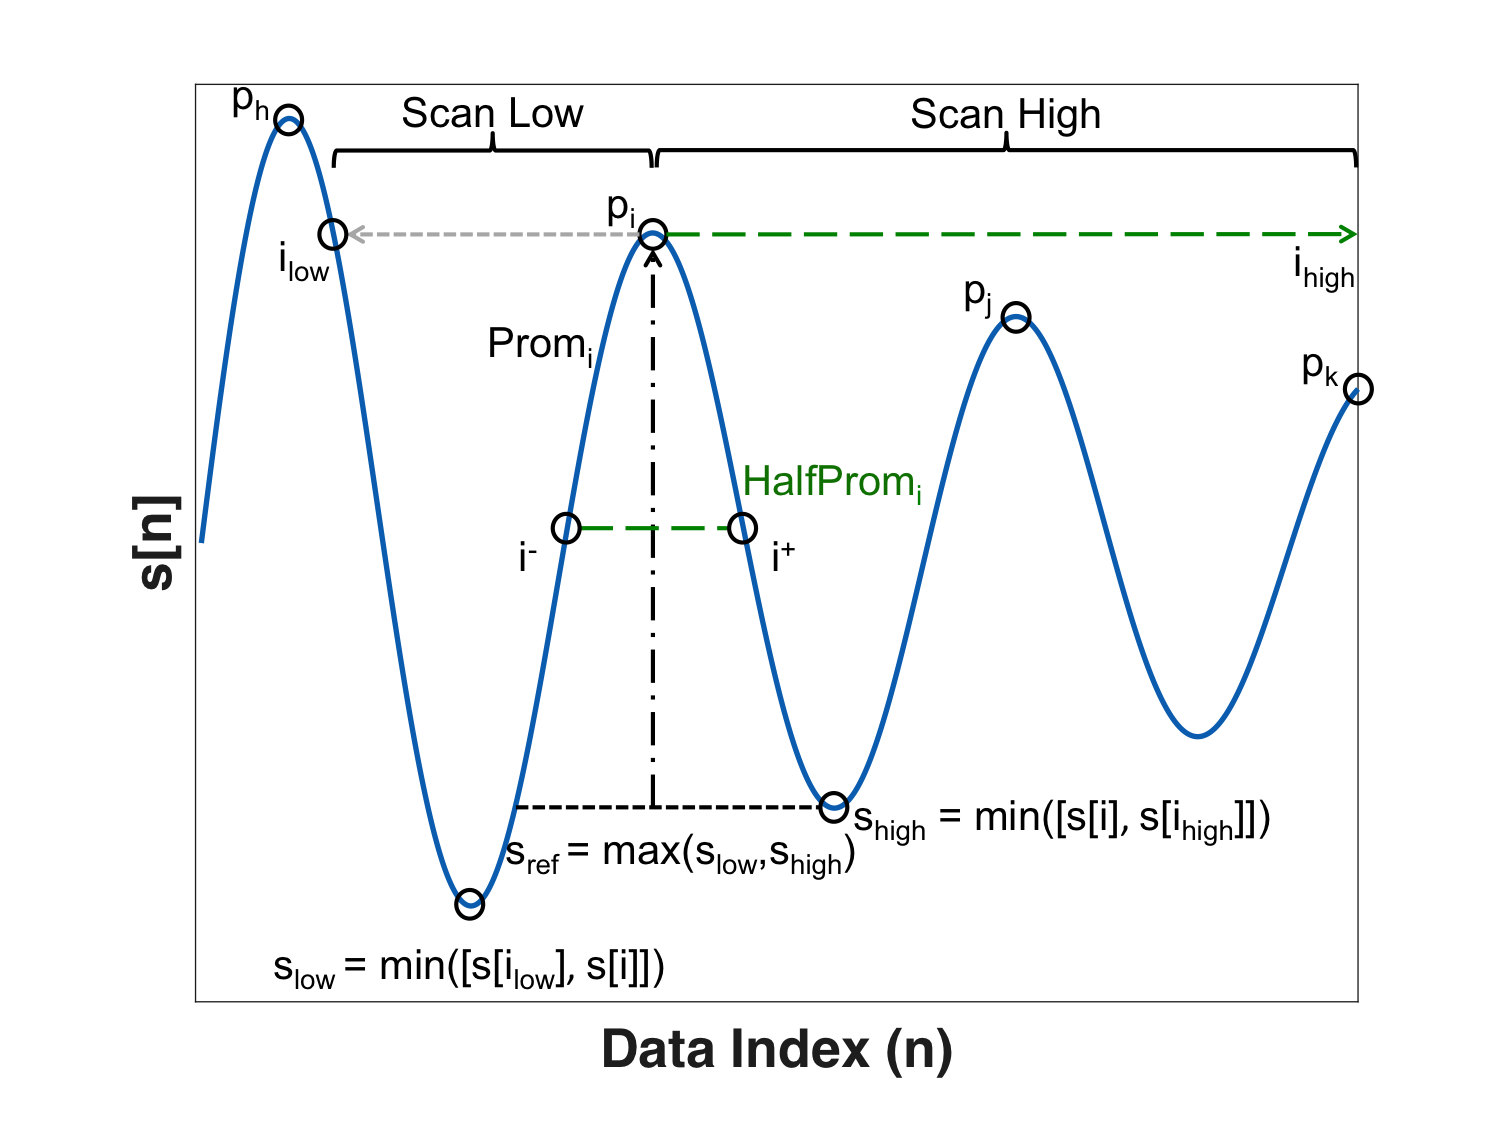
\includegraphics[width=12cm]{alg}
  \end{minipage}\hfill
  \caption[Algorithmic progression for calculating prominence]{Algorithmic progression. The blue, solid line represents a signal, $s[n]$, sampled at points, $n$, along the x-axis. Local maxima are labeled as points $p_{\{h,i,j,k\}}$. $s_{ref}$ marks the reference point from which the prominence, $Prom$, of peak $p_i$ is calculated. The width of the signal at the point of half-prominence, $HalfPromWidth$, is calculated by subtracting $i^-$ from $i^+$.}
	\label{fig:algProg}
\end{figure}

\subsection{Transducer Drive}
\label{ssec:MoM}

%The two measures of merit used in this study are average dissipated power of the transducer and volumetric flow rate of a clinical sample. Minimizing the transducer's power requirement via a geometry with an optimized resonance profile is desirable as high power requirements can result in localized heat buildup and chip failure. Maximizing volumetric flow rate allows for more rapid sample enrichment.

%\textbf{TODO Charlie: Add verbiage as to why we use Power as a measure of merit (tie displacement to power)}

The sinusoidal signal used to drive the transducer is generated by a function generator (AFG3022C, Tektronix, Beaverton, OR, USA) and amplified using a broadband RF amplifier (AG1021, T\&C Power Conversion, Rochester, NY, USA). The instantaneous voltage and current across the transducer is monitored using an oscilloscope (DPO2024B, Tektronix, Beaverton, OR, USA). In order to determine the actual power consumed by the transducer, it is first necessary to consider the instantaneous power as follows:

\begin{equation}
\label{eqn:instpower}
\hfill P_{inst} = VI = V_{max}sin(\omega t) I_{max} sin(\omega t-\varphi),\hfill
\end{equation}

\noindent where $V_{max}$ and $I_{max}$ are the maximum values of voltage and current, $\varphi$ is the phase lag between the instantaneous current and voltage signals, and $\omega=2\pi f$ is the sinusoidal drive frequency in rad/s. Using trigonometric identities and integrating over a cycle of the sinusoid we compute the average consumed power as:

\begin{equation}
\label{eqn:avgpower}
\hfill P_{avg} = V_{rms}I_{rms}cos\varphi,\hfill
\end{equation}

\noindent where $V_{rms}$ and $I_{rms}$ are the root mean square values of voltage and current. Using the oscilloscope, we multiply the instantaneous voltage and current and compute the average of this product to find the average consumed power in real time throughout our experiments.

Voltages and currents used to achieve 1 W of dissipated power at resonant frequencies for the baseline geometry and Chip 2.0 are shown in Table \ref{tab:comparison}. Note that the drive is not optimized for impedance matching, therefore most power is reflected.
\subsection{Blood Sample Preparation}
All experiments in this study used de-identified fresh human whole blood purchased from a vendor (Research Blood Components, Brighton MA), anticoagulated with acid–citrate–dextrose. In each case, the blood was diluted to 5\% by volume (for rapid screening tests) or 5\% hematocrit (for all other tests) in phosphate buffer solution (PBS 7.4 pH Lot Number 1832496). Cellular concentrations were measured before and after dilution using an automated hematology analyzer (XP-300, Sysmex Co., Kobe, Japan). The diluted sample was then transferred to a 10 ml plastic syringe (BD 10 ml Luer-Lok tip syringe 309604) and introduced to the chip through PVC tubing. The volumetric flow rate was regulated by a syringe pump (PhD Ultra, Harvard Apparatus).

\subsection{Bacteria--Blood Sample Preparation}

\textit{Pseudomonas aerouginosa}  was incubated overnight in a Lysogeny Broth (LB) culture. It was diluted by a factor of 50 and incubated until it reached a mid log phase. A whole blood sample was diluted into PBS as described in Section \ref{ssec:bloodAssay}. The optical density of the \textit{Pseudomonas} culture was taken and the appropriate dilution was calculated to create solution consisting of whole blood diluted in PBS to 5\% hematocrit and $10^5$ \textit{Pseudomonas} cells/ml. 

\subsection{Sample Measurement}
\label{sec:sampleMeasurement}

Blood or blood bacteria solutions were pumped through the device at its previously determined resonant frequency.  For each device this was found visually by observing the focusing stream--the most compact stream reveals the resonant frequency.  Outlet samples were collected in conical tubes after which they were measured and weighed for flow fraction and cell quantity calculations. 

Blood content was measured via a hematology analyzer while bacterial content was measured through a plating analysis: the samples were weighed, then serially diluted in 10x steps into PBS. Each dilution was cultured onto a plate of LB agar and incubated at 37$^{\circ}$C overnight after which the CFU were counted.   

The setpoint for 90\% RBC separation for variable power and fixed flow (50 $\mu$l/min) rate was accomplished by increasing power in small increments. Samples were collected from each output port and RBC counts were measured after each power increment. This process was repeated until a 90\% RBC separation ratio was achieved between the side and center ports.
%; smaller power increments were used to provide better resolution in determining the power conditions resulting in a separation ratio of 90\%. 

Determining 90\% RBC separation for variable flow rate and fixed power (1 W) required that the flow rate be set to 25 $\mu$l/min and increased in increments until such a point as 90\% RBC separation was achieved.  

\section{Results}
\label{sec:results}
\subsection{Screening Design of Experiments}
\label{ssec:doe}
Experiments must be initialized such that the sampling of the solution space can detect curvature in the response, as described in Section \ref{ssec:seeding}. Curvature in the response surface for an explanatory variable implies the existence of a local maxima in performance. Driving the design towards that local maxima is accomplished by isolating the variable in question and conducting experiments at adjacent points on the response plane, as outlined in Section \ref{ssec:iso}. 

Figure \ref{fig:geometry} illustrates the explanatory variables studied. Channel Width ($W_c$), channel height ($H_c$), side-wall width ($W_s$) and the position of the channel on the $y$-axis in two dimensional space ($Y_{pos}$) were selected as variables to study because they account for a majority of the two-dimensional design-space and are simple to vary during fabrication.

\subsection{Seeding of the Design Space (Rapid Screening Test)}
\label{ssec:seeding}

\begin{figure}[htb]
  \begin{minipage}[t]{0.99\linewidth}\centering
    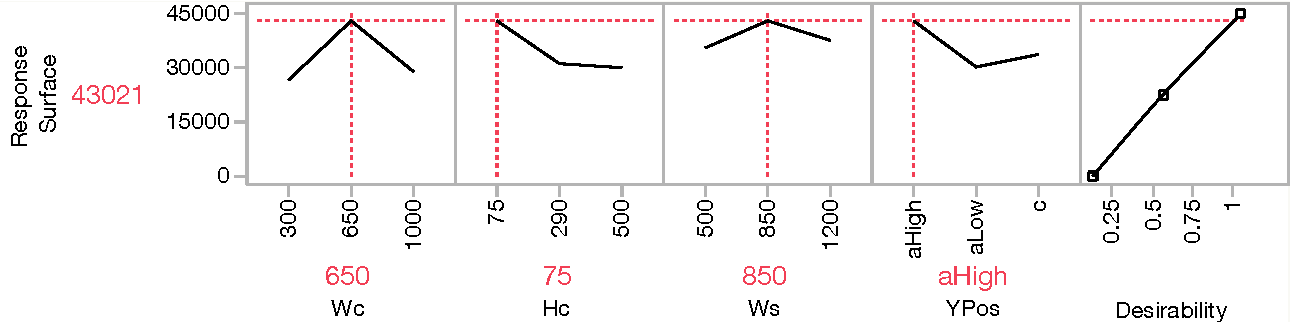
\includegraphics[width=14cm]{L9}
  \end{minipage}\hfill
  \caption[Results of initial seeding of design space]{Results of design space seeding. The quantities on the vertical axis correspond to the prominence data shown in Table \ref{tab:geometries}. The response surface is determined through a least squares fit of the aforementioned prominence values in four-dimensional space. The red dashed lines demarcate the points of maximum desirability.}
	\label{fig:L9}
\end{figure}

In order to economize the number of rapid screening experimental runs, an orthogonal array was chosen to generate a useful parameter set for the initial experiments. Orthogonal arrays are are used in design optimization to provide the most coverage of the solution space while minimizing the number of experimental runs \cite{yokoyama1993taguchi}. This is accomplished through the creation of an experimental set such that each combination of the array's strength appears equally often \cite{hedayat2012orthogonal}. The orthogonal array used to seed the design space is known as the $L_9 (3^4)$ array, which has a strength of two and is used to probe a solution space consisting of four explanatory variables at three settings in nine experimental runs, as opposed to the 81 experimental runs required to conduct the full-factorial experiment \cite{hedayat2012orthogonal}. The use of three explanatory variable settings was chosen in order to detect curvature in the response surface. The parameter set tested while seeding the design space, in accordance with an $L_9 (3^4)$ orthogonal array, is shown in Table \ref{tab:geometries}.

%Since the parameters generated during the initial seeding of the design space cannot assume a functional geometry (i.e., a geometry capable of focusing blood), the purpose of the initial iteration of experiments is directed towards discovering functional designs, as opposed to a comparison between functional designs. As such, the performance parameter used during this initial phase is peak prominence (Figure \ref{fig:algProg}c.). This is because $\chi$ (Figure \ref{fig:algProg}d.) can skew the results by rewarding peaks with small prominence values (i.e., poor focusing) and correspondingly small widths.  

\begin{table}[h]
% table caption is above the table
\caption[Geometries tested for L9 design array]{Geometries tested for L9 design array with corresponding Chip ID. All dimensions are given in units of $\mu$m. Prominence values are given in units of pixel intensity and correspond to each chip's maximum prominence value for the tested bandwidth. The given frequencies indicate the point at which the maximum prominence was observed.}
\label{tab:geometries}       % Give a unique label
% For LaTeX tables use
\centering
\begin{tabular}{lllll|cc}
\hline\noalign{\smallskip}
ID & $W_c$ & $H_c$ & $W_s$ & $Y_{Pos}$ & Prominence & $f$ ($MHz$) \\
\noalign{\smallskip}\hline\noalign{\smallskip}
1L9 & 300 & 75 & 500 & Low & 6375 & 1.58\\
2L9 & 300 & 290 & 850 & Center & 5496 & 1.22\\
3L9 & 300 & 500 & 1200 & High & 8240 & 0.67\\
4L9 & 650 & 75 & 850 & High & 43021 & 0.55\\
5L9 & 650 & 290 & 1200 & Low & 12950 & 0.66\\
6L9 & 650 & 500 & 500 & Center & 13251 & 0.57\\
7L9 & 1000 & 75 & 1200 & Center & 14215 & 0.74\\
8L9 & 1000 & 290 & 500 & High & 9574 & 0.73\\
9L9 & 1000 & 500 & 850 & Low & 3144 & 0.71\\
\noalign{\smallskip}\hline
\end{tabular}
\end{table}

The response surface generated from the data points shown in Table \ref{tab:geometries} was analyzed using statistical software (JMP®, Version 13.0.0. SAS Institute Inc., Cary, NC, 1989-2017) and is shown in Figure \ref{fig:L9}. Maximum desirability of the performance parameter (prominence) is achieved by setting $W_c$ to 650$\mu$m, $H_c$ to 75$\mu$m, $W_s$ to 850$\mu$m and placing the channel in the high vertical position (i.e., Chip 4L9 in Table \ref{tab:geometries}). Additionally, the response surface shows significant curvature while modulating the width of the channel, leading into the next iteration of the study outlined in Section \ref{sssec:width}.

\subsection{Variable Isolation Studies}
\label{ssec:iso}

\subsubsection{Channel Width Study (Rapid Screening Test)}
\label{sssec:width}

Proceeding from the  results of the initial seeding of the design space,  we fixed the other parameters from the best geometry (4L9) and varied the channel width in 50$\mu$m increments.  Although the response surface indicates that thinner channel height may be preferable,  we selected a height of 100$\mu$m for this variable isolation study, anticipating that a slightly greater channel height would have practical advantages. 

\begin{table}[h]
% table caption is above the table
	\caption[Geometries tested for an isolation study of channel width]{Geometries tested for an isolation study of channel width with corresponding Chip ID. All dimensions are given in units of $\mu$m. Prominence values are given in units of pixel intensity and correspond to each chip's maximum prominence value for the tested bandwidth. The given frequencies indicate the point at which the maximum prominence was observed. The frequency range scanned spanned from 500 kHz to 2 MHz. No focusing was observed within this range for the design with a channel width of 700$\mu$m. }   
\label{tab:width}       % Give a unique label
% For LaTeX tables use
\centering
\begin{tabular}{lllll|cc}
\hline\noalign{\smallskip}
ID & $W_c$ & $H_c$ & $W_s$ & $Y_{Pos}$ & Prominence & $f$ ($MHz$)\\
\noalign{\smallskip}\hline\noalign{\smallskip}
1Wc & 500 & 100 & 850 & High & 12143 & 0.64\\
2Wc & 550 & 100 & 850 & High & 15200 & 0.51\\
3Wc & 600 & 100 & 850 & High & 4770 & 1.58\\
4Wc & 650 & 100 & 850 & High & 5470 & 1.99\\
5Wc & 700 & 100 & 850 & High & - & - \\
\noalign{\smallskip}\hline
\end{tabular}
\end{table}

As shown in Table \ref{tab:width}, the highest performing channel width, holding other factors constant, was 550$\mu$m. Channels having a width of 600$\mu$m and above demonstrated the ability to focus RBCs to the center fifth of the channel, however the focusing was a result of driving the chip at a higher order mode thus creating more than one focusing band across the channel width. 

As a significant performance shift was observed as a result of a small adjustment to $H_c$, channel height was chosen as the variable to isolate for the next design set. 

\subsubsection{Channel Height Study (Final Screening Test)}
\label{sssec:height}

This design set fixed values for $W_c$, $W_s$, and $Y_{Pos}$ while varying $H_c$ resulting in the geometries shown in Table \ref{tab:height}. All devices in this set demonstrated focusing of blood; the frequencies for which are shown in Table \ref{tab:height}. This study was conducted in accordance with the final screening test specified in Section \ref{sssec:finalScreen}. The results shown in Figure \ref{fig:heightPlot} demonstrate that, for flow rates higher than 25 $\mu$l/min, the chip with a channel height of 250$\mu$m performed better than the other chips tested in terms of $\chi$ at all studied power levels. Thus the winning geometry of the study's device screening stage has a channel width of 550$\mu$m, a channel height of 250$\mu$m, a side-wall width of 850$\mu$m, with the channel in the High vertical position (i.e., Chip 4Hc in Table \ref{tab:height}).

\begin{figure}[H]
  \begin{minipage}[t]{0.49\linewidth}\centering
    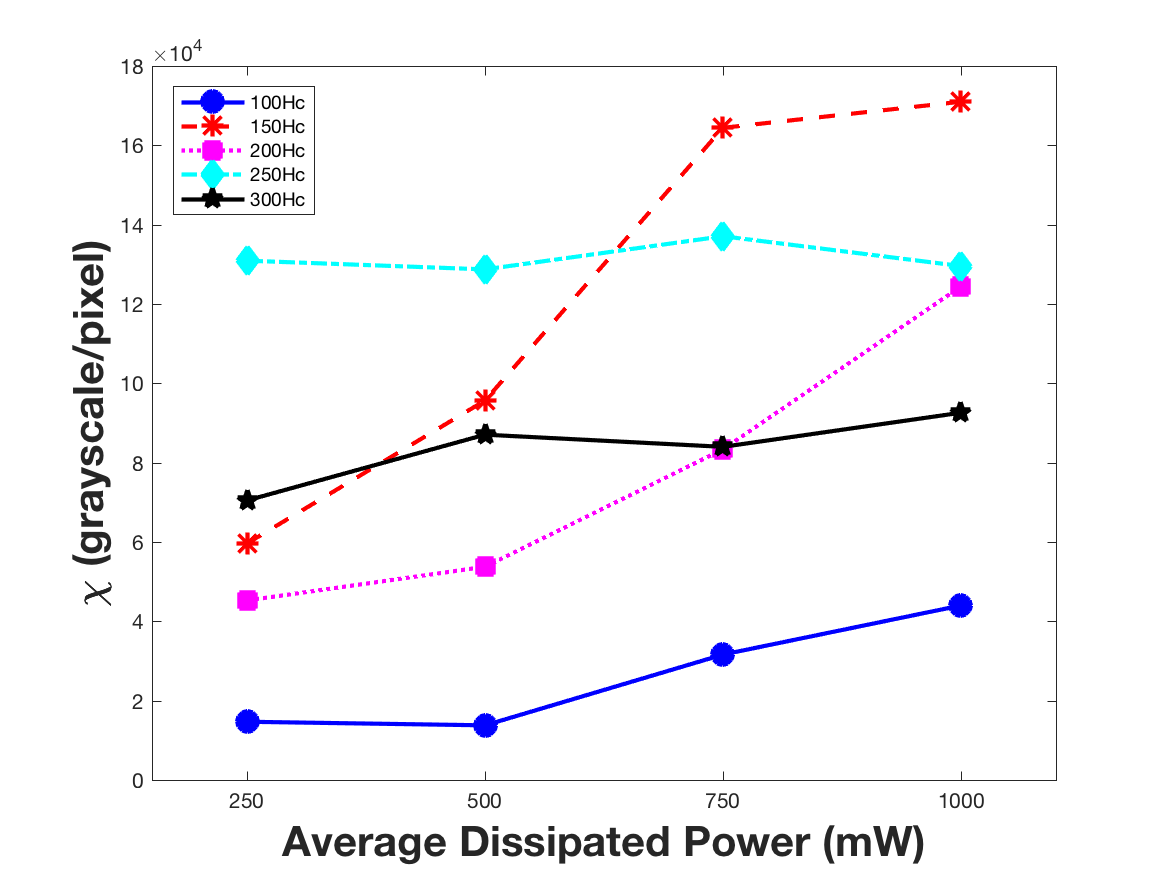
\includegraphics[width=7cm]{HeightPlot25ul}
    \medskip
    \centerline{(a) 25 $\mu$l/min}
  \end{minipage}\hfill
  \begin{minipage}[t]{0.49\linewidth}\centering
    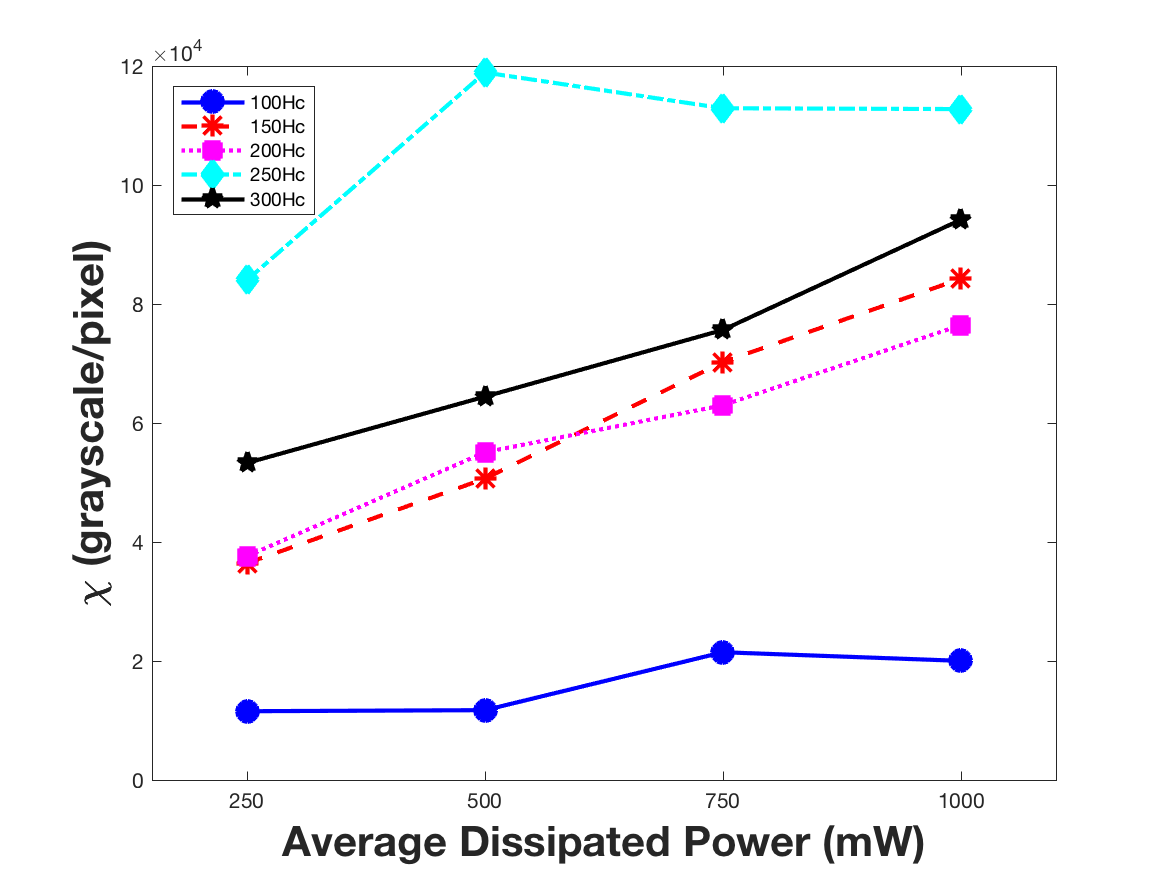
\includegraphics[width=7cm]{HeightPlot50ul}
    \medskip
    \centerline{(b) 50 $\mu$l/min}
  \end{minipage}
  \begin{minipage}[t]{0.99\linewidth}\centering
    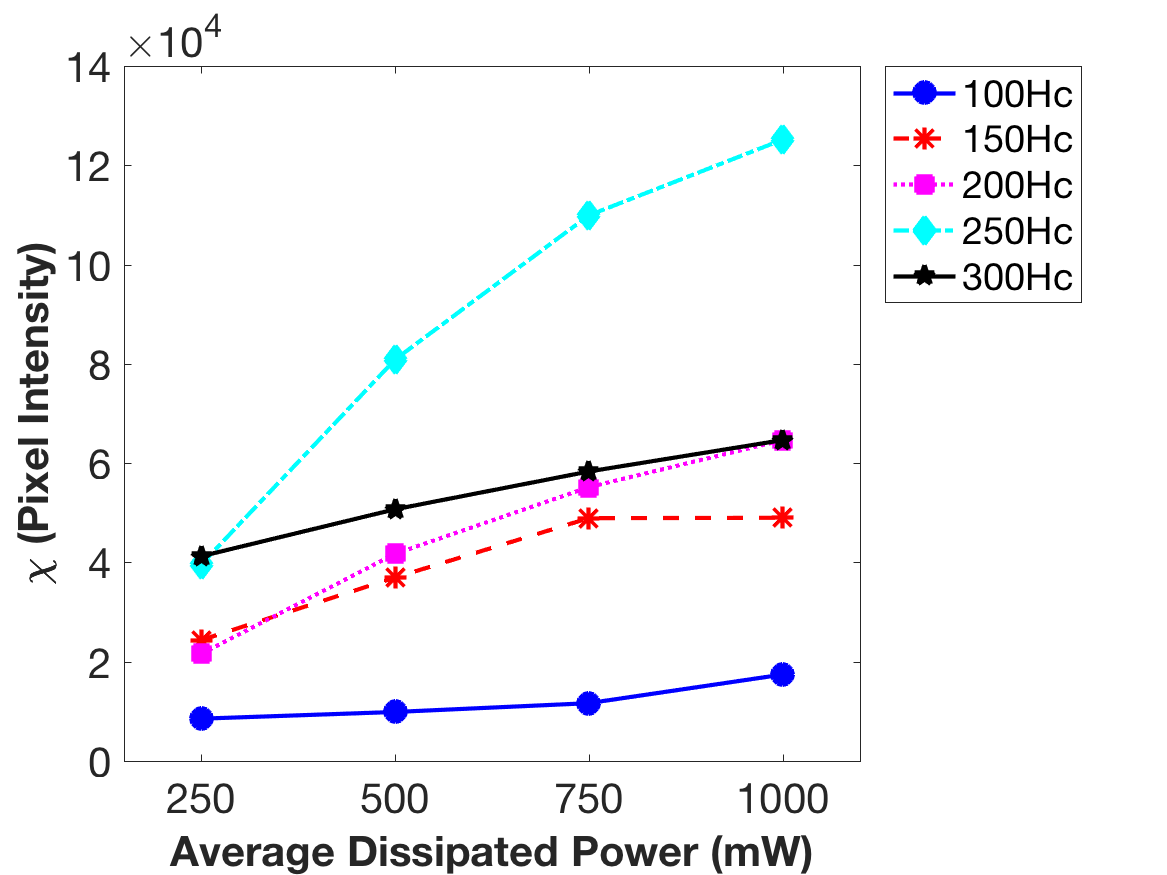
\includegraphics[width=7cm]{HeightPlot75ul}
    \medskip
    \centerline{(c) 75 $\mu$l/min}
  \end{minipage}
  \caption[Performance comparison of channel height study using image analysis]{Performance comparison of channel height study using image analysis. (a-c) plot the performance of the geometries in Table \ref{tab:height} for three volumetric flow rates: 25 $\mu$l/min, 50 $\mu$l/min and 75 $\mu$l/min, respectively. Performance is calculated from microscope images in the manner described in Section \ref{ssec:promToWidth}.  Datasets are shown for each channel height from 100 to 300$\mu$m.}
	\label{fig:heightPlot}
\end{figure}



\begin{table}[h]
% table caption is above the table
\caption[Geometries tested for a final screening study of channel height]{Geometries tested for a final screening study of channel height with corresponding Chip ID. All dimensions are given in units of $\mu$m. The listed frequencies coincide with the locations of the corresponding device's fundamental odd resonant mode.}
\label{tab:height}       % Give a unique label
% For LaTeX tables use
\centering
\begin{tabular}{lllll | c}
\hline\noalign{\smallskip}
ID & $W_c$ & $H_c$ & $W_s$ & $Y_{Pos}$ & $f$ ($MHz$)\\
\noalign{\smallskip}\hline\noalign{\smallskip}
1Hc & 550 & 100 & 850 & High & 0.684 \\
2Hc & 550 & 150 & 850 & High & 0.640 \\
3Hc & 550 & 200 & 850 & High & 0.634 \\
4Hc & 550 & 250 & 850 & High & 0.632 \\
5Hc & 550 & 300 & 850 & High & 0.640 \\
\noalign{\smallskip}\hline
\end{tabular}
\end{table}

\subsection{Comparison of Chip 2.0 versus Baseline Geometry}
\label{ssec:comparison}

The results of the screening tests shown in Figure \ref{fig:heightPlot} yield a geometry that outperformed the other devices in terms of RBC focusing analyzed by image analysis. However, in order to gauge the ultimate success of this geometry it was tested against the baseline geometry. This section presents results from three experiments that compared the winning geometry of the screening tests (i.e., Chip 2.0) against the baseline geometry through image analysis, blood separation, and bacteria separation.

\begin{table}[t]
% table caption is above the table
	\caption[Standard operating conditions for Baseline versus Chip 2.0]{Baseline versus Chip 2.0. All dimensions are given in units of $\mu$m. Standard operating conditions, measured at the transducer, are provided for frequencies, input voltages and currents required to achieve 1 W of average dissipated power. These conditions are the values for which the fundamental resonant odd modes for each chip were achieved.}
\label{tab:comparison}       % Give a unique label
% For LaTeX tables use
\centering
\begin{tabular}{lllll | ccc}
\hline\noalign{\smallskip}
Chip & $W_c$ & $H_c$ & $W_s$ & $Y_{Pos}$ & $f$ ($MHz$) & Voltage ($V_{pp}$) & Current ($mA_{pp}$) \\
\noalign{\smallskip}\hline\noalign{\smallskip}
Chip 2.0 & 550 & 250 & 850 & High & 0.632 & 56.44 ($\pm$2.4) & 1039 ($\pm$53)\\
Baseline & 430 & 200 &  1055 & High & 1.012 & 45.78 ($\pm$1.86)& 1340 ($\pm$70)\\ 
\noalign{\smallskip}\hline
\end{tabular}
\end{table}

\subsubsection{Comparative Focusing}
\label{sssec:comparisonFocusing}

\begin{figure}[H]
  \begin{minipage}[t]{0.49\linewidth}\centering
    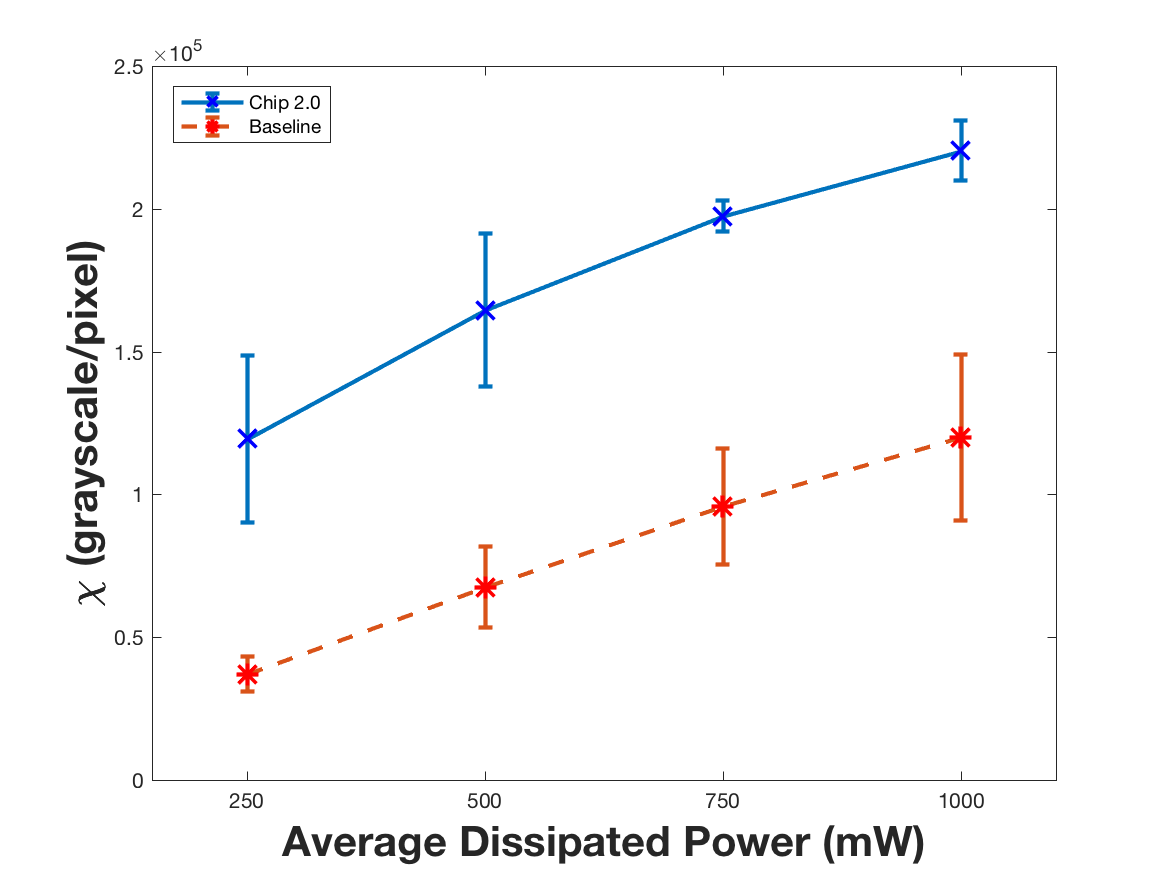
\includegraphics[width=7cm]{ErrorBars25ul}
    \medskip
    \centerline{(a) 25 $\mu$l/min}
  \end{minipage}\hfill
  \begin{minipage}[t]{0.49\linewidth}\centering
    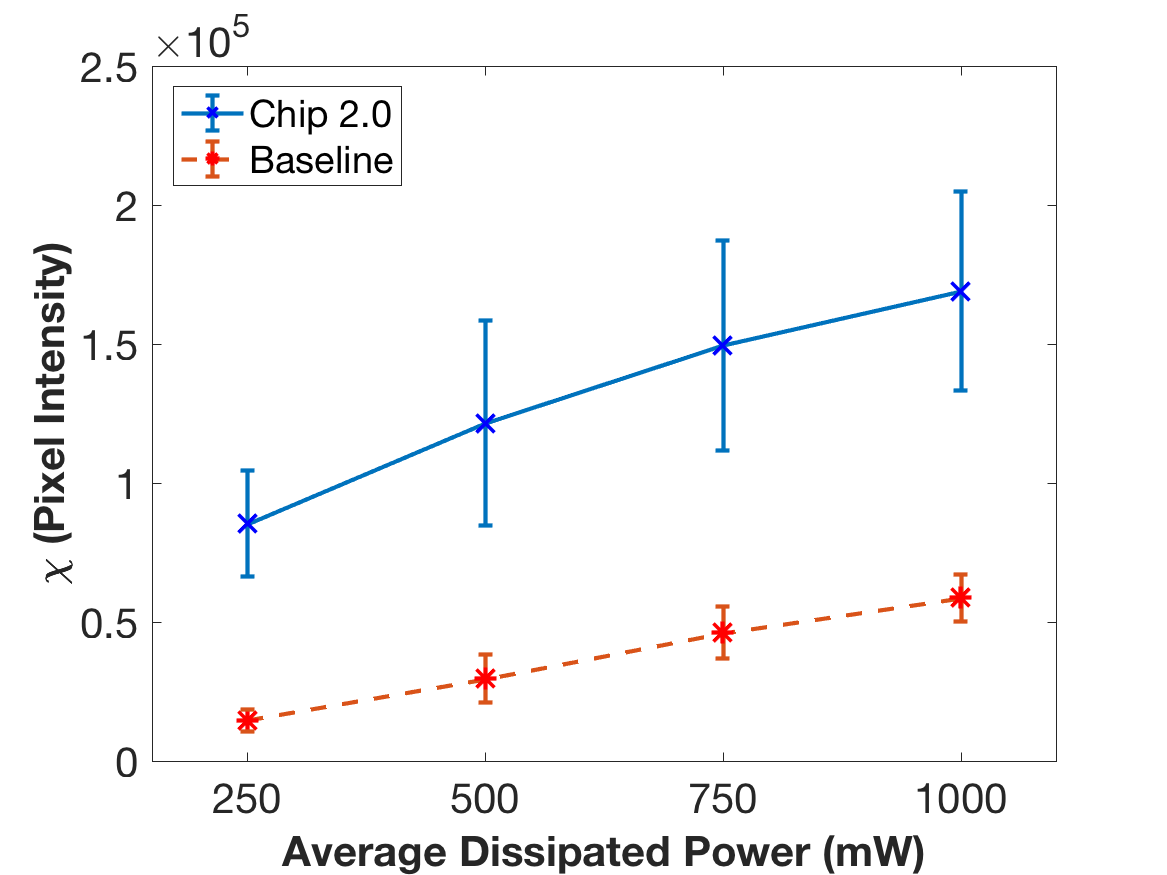
\includegraphics[width=7cm]{ErrorBars50ul}
    \medskip
    \centerline{(b) 50 $\mu$l/min}\\
  \end{minipage}
  \begin{minipage}[t]{0.99\linewidth}\centering
    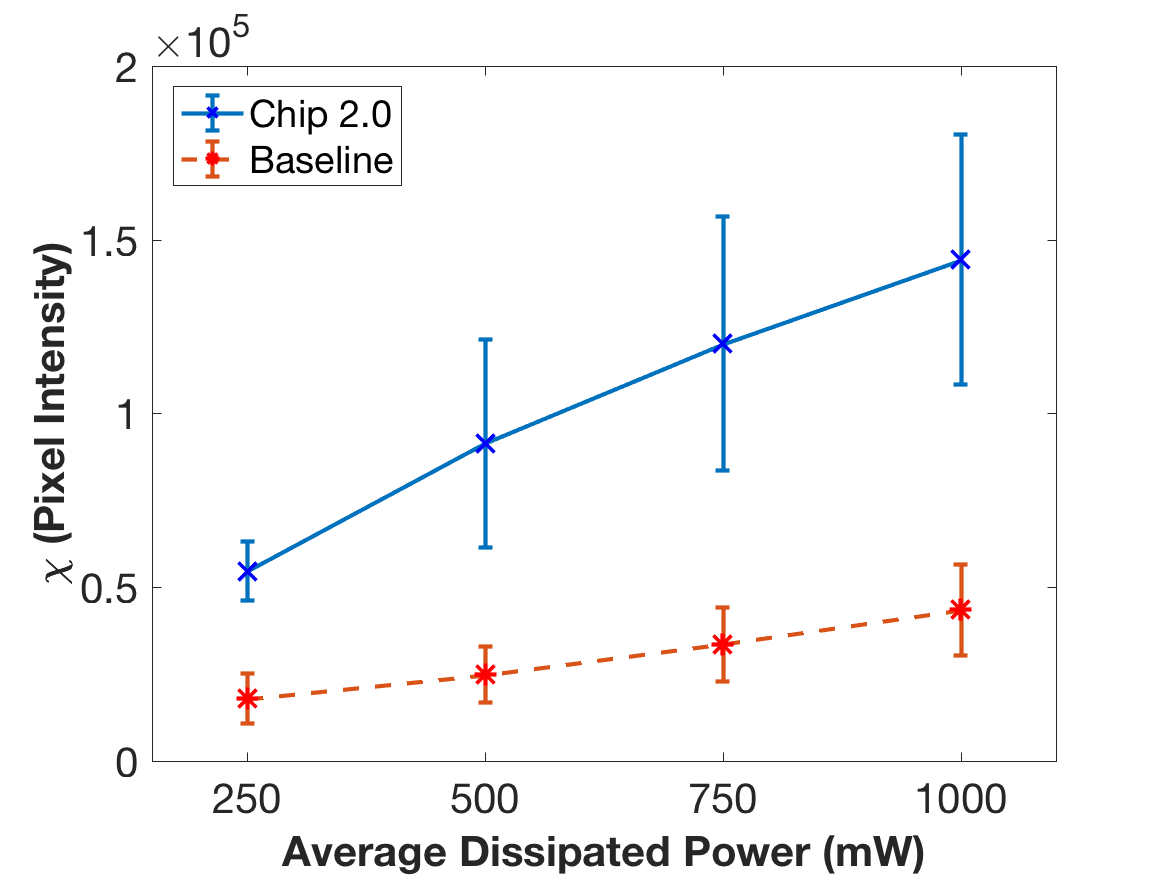
\includegraphics[width=7cm]{ErrorBars75ul}
    \medskip
    \centerline{(c) 75 $\mu$l/min}
  \end{minipage}
  \caption[Performance comparison versus baseline using image analysis]{Performance comparison versus baseline using image analysis. (a-c) plot the performance of the baseline versus the winner of the study for three volumetric flow rates: 25 $\mu$l/min, 50 $\mu$l/min and 75 $\mu$l/min, respectively. Performance is calculated from microscope images in the manner described in Section \ref{ssec:promToWidth}.}
	\label{fig:headToHeadImages}
\end{figure}


Figure \ref{fig:headToHeadImages}(a--c) plots the performance of Chip 2.0 against the baseline in terms $\chi$. The results show that Chip 2.0 outperforms the baseline for all tested combinations of flow and power settings.
\subsubsection{Comparative Blood Separation}
\label{sssec:comparisonBlood}

\begin{figure}[H]
  \begin{minipage}[t]{0.49\linewidth}\centering
    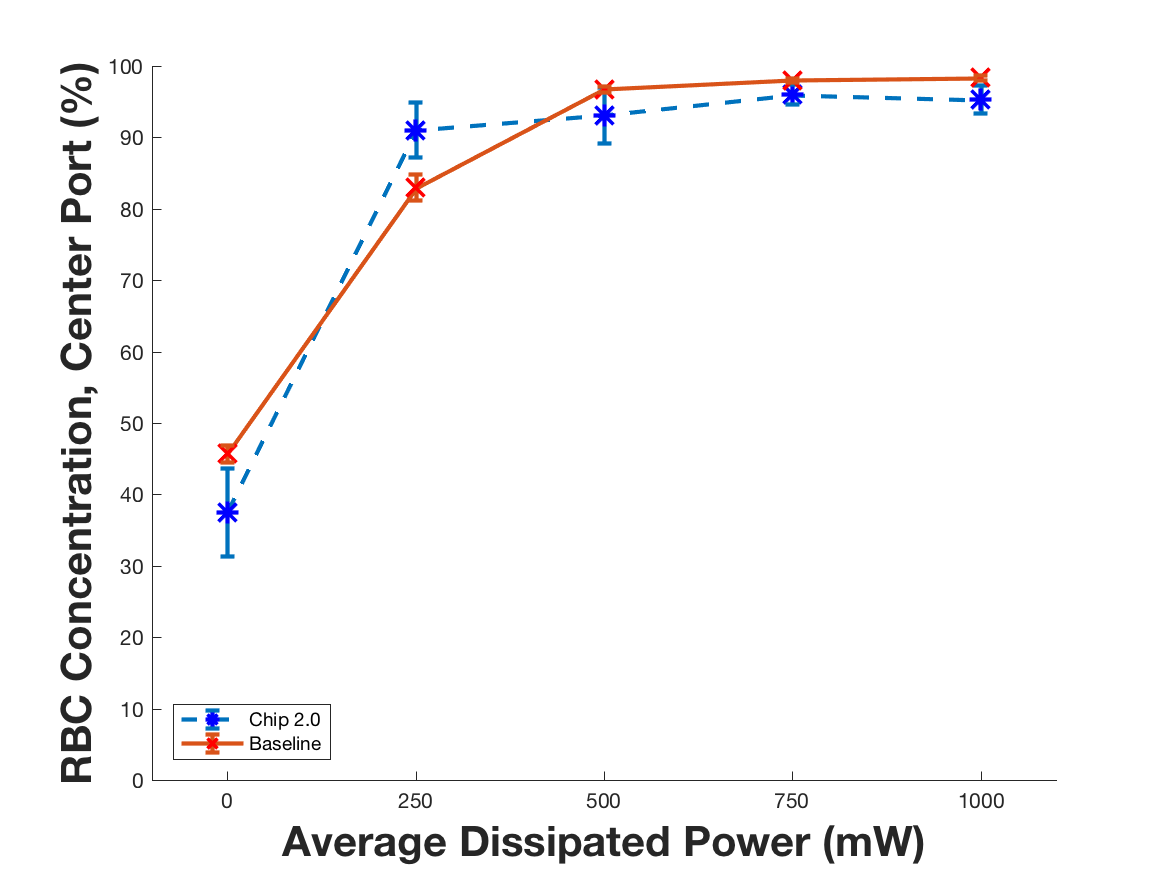
\includegraphics[width=7cm]{ErrorBarBloodData25ul}
    \medskip
    \centerline{(a) 25 $\mu$l/min}
  \end{minipage}\hfill
  \begin{minipage}[t]{0.49\linewidth}\centering
    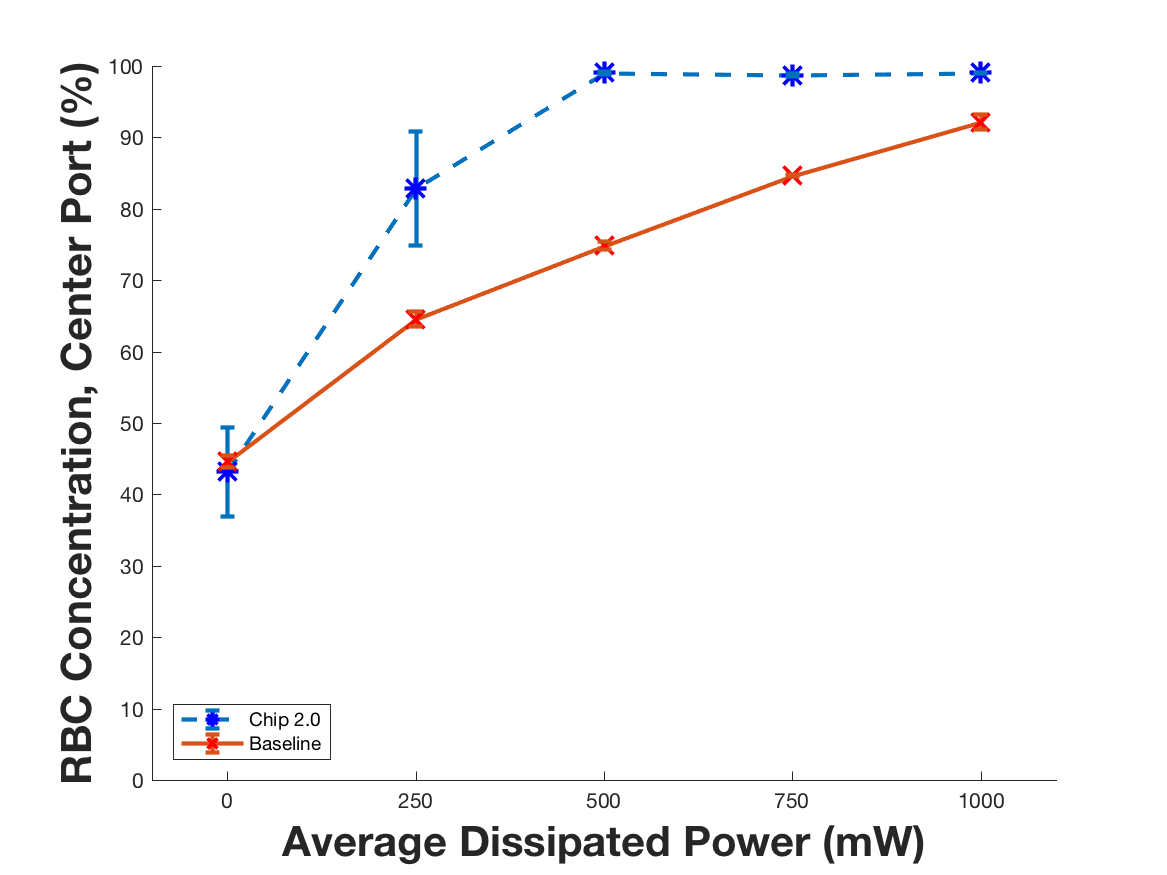
\includegraphics[width=7cm]{ErrorBarBloodData50ul}
    \medskip
    \centerline{(b) 50 $\mu$l/min}\\
  \end{minipage}
  \begin{minipage}[t]{0.99\linewidth}\centering
    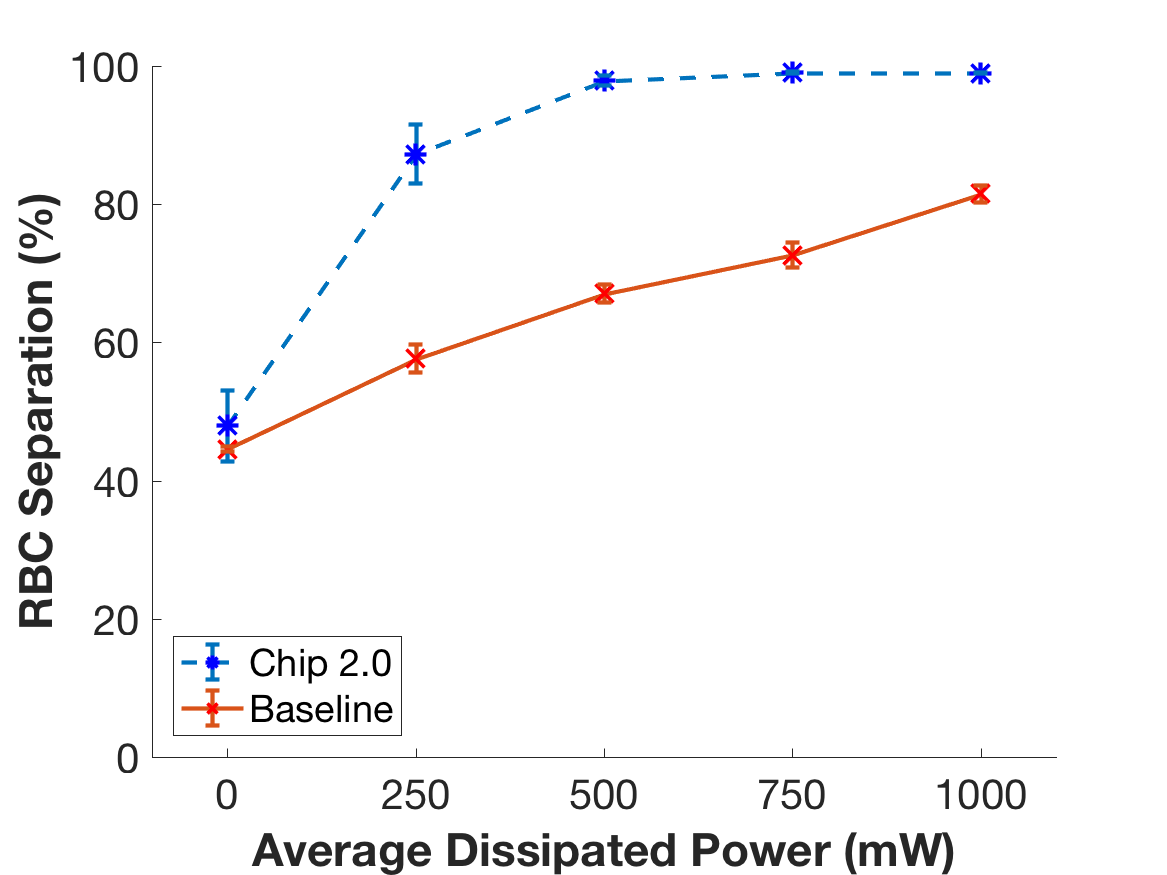
\includegraphics[width=7cm]{ErrorBarBloodData75ul}
    \medskip
    \centerline{(c) 75 $\mu$l/min}
  \end{minipage}
  \caption[Separation performance comparison versus baseline]{Blood separation performance comparison versus baseline. (a-c) plot the performance of the baseline versus the winner of the study for three volumetric flow rates: 25 $\mu$l/min, 50 $\mu$l/min and 75 $\mu$l/min, respectively. Performance is defined based on each design's ability to focus RBCs into the middle channel of the trifurcation shown in Figure \ref{fig:geometry}. RBC separation is defined as the number of RBCs measured at the center port divided by the total number of RBCs measured at the input port.}
	\label{fig:headToHeadBlood}
\end{figure}


Figure \ref{fig:headToHeadBlood} plots the performance of Chip 2.0 against the baseline in terms of each device's ability to focus RBCs to the center port. The dynamic range of each measurement was limited between the control measurement (i.e., zero average dissipated power) and 100\% RBC concentration in the center channel. As the chip has two outlet ports (Figure \ref{fig:geometry}), RBCs will be approximately equally distributed between them in the acoustics-off (0 W input power) condition. The baseline and Chip 2.0 demonstrated comparable performance at a flow rate of 25 $\mu$l/min across all power settings; however, at higher flow rates Chip 2.0 outperformed the baseline across all non-control power settings. 



\subsubsection{Comparative Bacterial Separation}
\label{sssec:comparisonBacteria}

Four experiments were conducted in three technical replicates, two for each device design (baseline and Chip 2.0),  in order to determine the optimal value for each measure of merit while holding the other constant. Optimality was defined as the maximum flow rate or minimum power required to maintain at least 90\% RBC separation between the side and center ports while bacteria recovery in the side port was measured. 

The results in Figure \ref{fig:bacPerf} show that Chip 2.0 achieved a 175\% increase in throughput relative to the baseline. Additionally, Chip 2.0 was able to decrease the average dissipated power by 81.63\% when compared to that of the baseline geometry. The actual average RBC separation across all four experiments was 95.25\% ($\pm$1.89\%). The yield of the bacterial samples collected at the side port had a standard deviation of 0.05\%.  For both devices the yield of bacteria in the side port was 33.5\% ($\pm$3\%) after separation, showing that separation performance in the 2.0 design is equal to that of the baseline while enabling lower driving power and/or higher throughput.

\begin{figure}[H]
  \begin{minipage}[t]{0.49\linewidth}\centering
    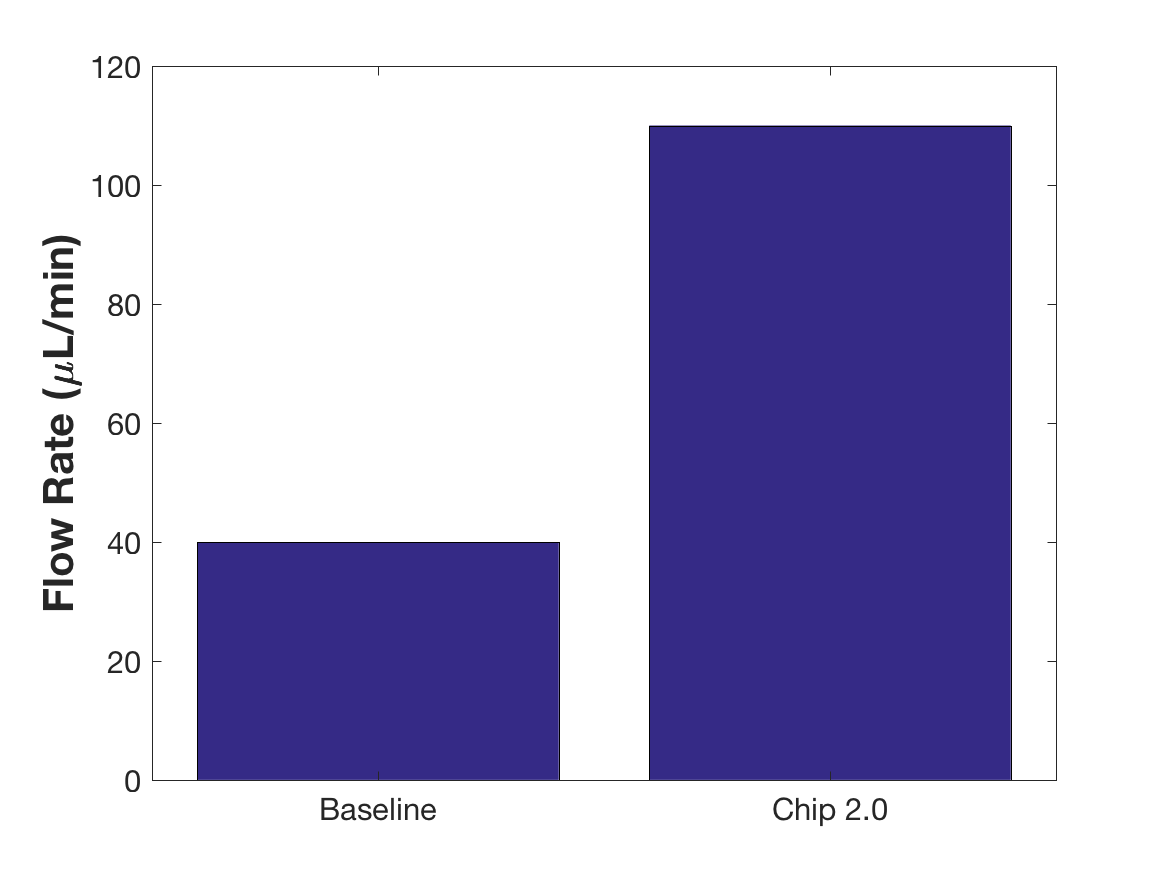
\includegraphics[width=7cm]{flowBac}
    \medskip
    \centerline{(a) Flow Rate at 1 W}
  \end{minipage}\hfill
  \begin{minipage}[t]{0.49\linewidth}\centering
    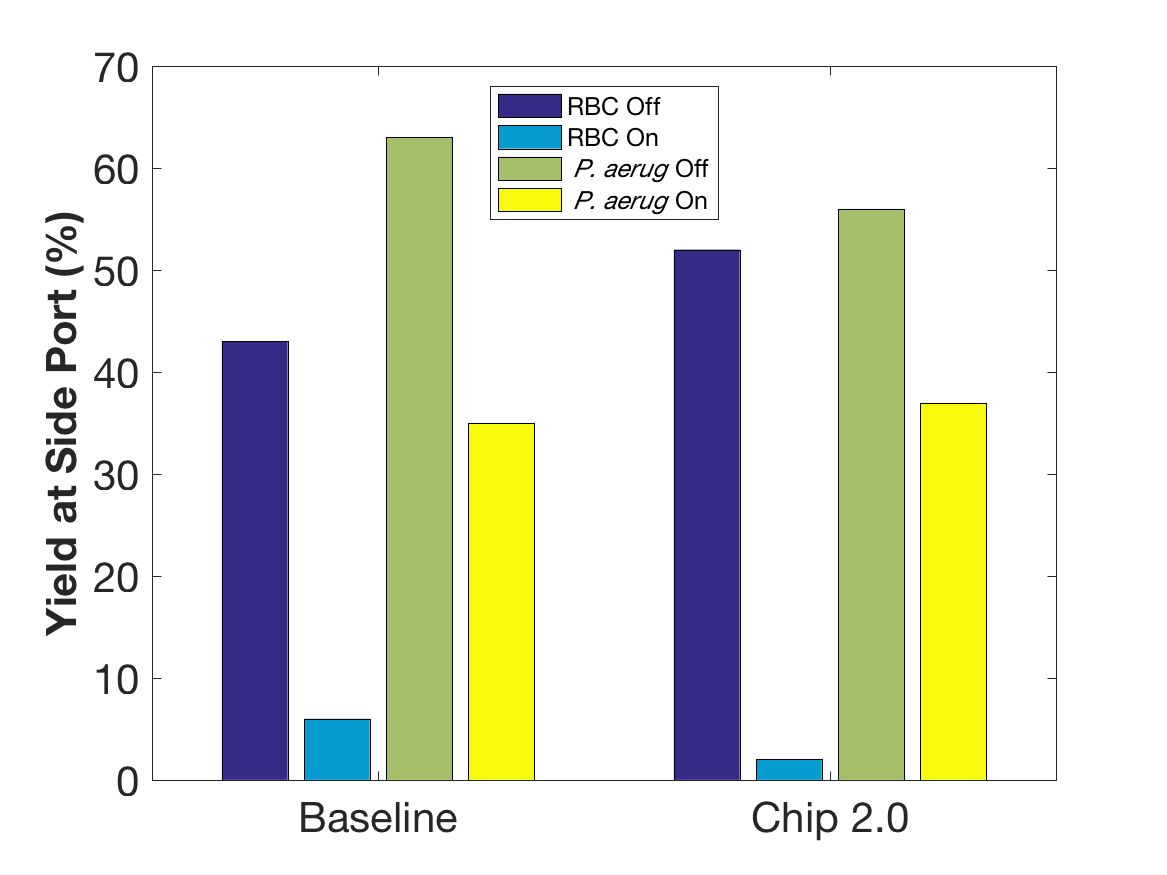
\includegraphics[width=7cm]{maxFlow}
    \medskip
    \centerline{(b) Separation performance for (a)}
  \end{minipage}\\
  \begin{minipage}[t]{0.49\linewidth}\centering
    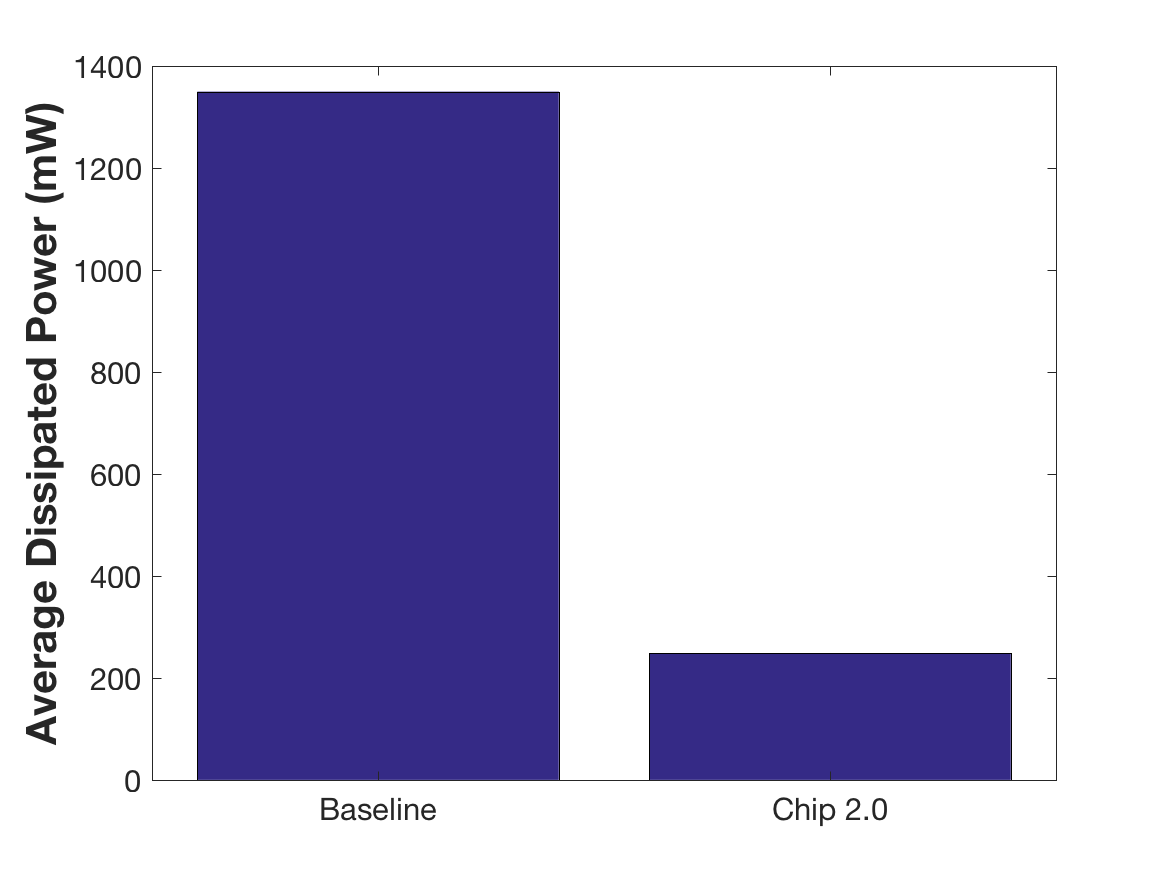
\includegraphics[width=7cm]{powerBac}
    \medskip
    \centerline{(c) Power at 50 $\mu$l/min}
  \end{minipage}\hfill
  \begin{minipage}[t]{0.49\linewidth}\centering
    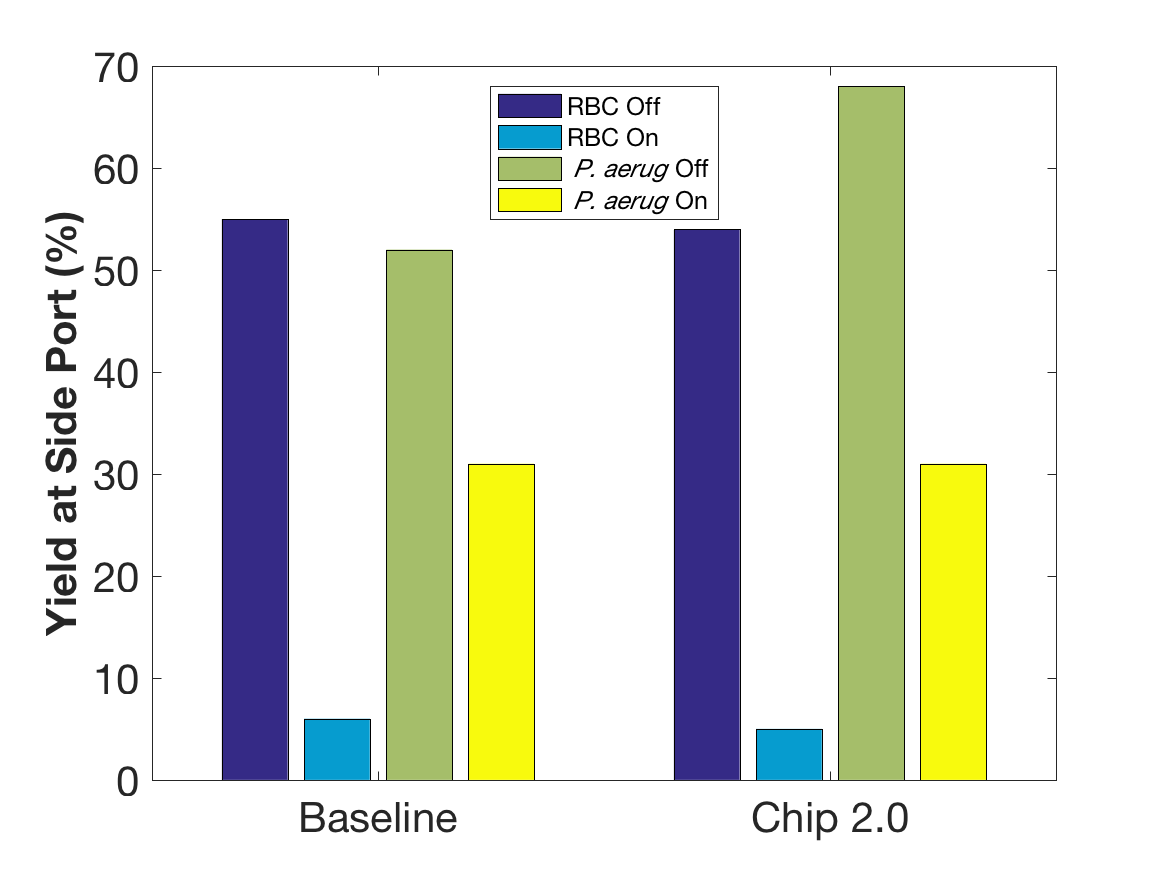
\includegraphics[width=7cm]{minPower}
    \medskip
    \centerline{(d) Separation performance for (b)}
  \end{minipage}\\
  \caption[Bacterial separation performance comparison]{Levels of each measure of merit required to achieve equivalent separation performance. (a) shows the relative performance of the baseline as it compares to Chip 2.0 in terms of flow rate with power held constant at 1 W. (b) illustrates the actual performance of each chip at the levels specified in (a) in both the acoustics ``off'' (0 W and established chip flow rate) and ``on'' conditions (1 W and established flow conditions). (c) summarizes the performance of the two chip designs holding flow rate at 50 $\mu$l/min while varying power. Constant values were maintained for RBC separation and bacterial recovery for all chip designs and experiments. (d) depicts the performance of each device at the power levels specified in (c); ``off'' being the control condition of 0 W and 50 $\mu$l/min.}
	\label{fig:bacPerf}
\end{figure}



It is worth noting that the Chip 2.0 design achieved better RBC separation  for both the maximum flow rate and minimum power experiments (98\% vs 94\% and 95\% vs 94\%, respectively) and equivalent bacterial recovery relative to the baseline across all four experiments; thus, for each Chip 2.0 experiment the measure of merit (flow or power) could show greater advantages if the RBC yield were adjusted to match that of the baseline. 

%Claim: without losing performance, we increased throughput and lowered power.

\section{Discussion}
\label{sec:discussion}

The resonant response of acoustophoretic microfluidic devices has been shown to be non-linear \cite{garofalo2016performance}\cite{bora2015efficient}\cite{glynne2009new}\cite{hahn2014modeling}. Complex response patterns with numerous explanatory variables have been successfully optimized using a fractional factorial experimental design approach in conjunction with a response surface methodology \cite{khuri2010response}; however, these methodologies assume that the function $f(x)$ modeling the response variable $y$ to the explanatory variables $x=(x_1,x_2,\dots,x_n)$ accounting for some experimental error $\epsilon$, as shown in Equation \ref{eqn:response}, is a low-degree polynomial \cite{khuri2010response}, 

\begin{equation}
\label{eqn:response}
  \hfill y=f(x)+\epsilon \hfill
\end{equation}

In the absence of a near-quadratic response, multiple rounds of experiments are required to adequately detect a positive gradient in performance \cite{carley2004response}. Even after multiple rounds of experiments, the nature of a complex response surface means that no claim of optimality can be made \cite{box2006improving}. Since this study seeks a performance enhancement, as opposed to a rigorous optimal geometry, this iterative method is acceptable.   

This study successfully improved the performance of the acoustic separator chip for both measures of merit. However, Chip 2.0 may not represent an optimal design, and further improvement is likely possible.  The experimental design selected parameters that were most accessible to systematic variation.  For example, the impact of total height of the device was not explored because changes in sheet stock thickness would require sourcing or custom fabricating those sheets, and the bond process would have to be adjusted for each thickness.  Likewise, the selection of the values tested assumes a more or less smoothly varying response.  Further analysis is needed to rigorously support that assumption.   

The frequency range studied for the rapid screening tests (0.5 -- 2.0 MHz) was chosen based on the known resonance of the baseline device (approximately 1 MHz) and the expectation that small variations in dimensions should result in comparably small variations in resonant frequency.  Additionally, the lower limit was selected with the knowledge that acoustic radiation force scales with frequency and lower frequencies could limit the ability of the device to focus small cells or particles such as platelets or bacteria, if desired in other applications.  Furthermore, there were practical experimental limitations at the upper end of the range; a transducer with a higher resonant frequency (e.g., 5 MHz) would allow a wider range of frequencies to be explored, however the fragility of such transducers increases the difficulty of mounting and testing the devices.  Nevertheless reproducing the screening with a wider frequency range, particularly at the low end could yield further improvements.


Despite these and other limitations, this study was meant not only to identify an improved geometry, but also to establish a method for empirical development of devices.  The resulting performance improvement, as measured by the bacteria separation task, suggest that the initial screening using only image-based analysis of RBC focusing provides a useful approach for assessing devices.  To perform the setup, operation, output sample collection, and cell counting in the final bacteria separation takes several hours at least with all parameters fixed, whereas hundreds of image-based prominance measurements could be made at a rate of one every 15 seconds. 

Future explorations of device designs can be enabled by this parametric, rapid prototyping framework, which is part of a larger workflow \cite{ali2017iwbda}\cite{lippai2017iwbda}\cite{krishna2017iwbda}. The 19 devices designed in this manuscript can take advantage of this process with a high level description of the device functionality, microfluidic primitives, and automated fabrication and control.

%The accuracy of the desktop micromill ($<$0.003" per 6" of linear travel \cite{othermill}) as well as the centerline deviation (TIR) of the tools used to machine the chips all functioned within published parameters. This was confirmed using a calibrated microscope and drop gauge (\textbf{\uppercase{I need to grab the model number from the machine shop}}). YOU CAN TAKE THIS OUT OR MOVE TO METHODS

%Finally, many unstudied parameters exist upon which another optimization effort can be conducted. As this study only used one type of transducer, one can imagine another study sweeping across the mechanical quality factor ($Q_m$), resonant frequency, size, or material of the piezoelectric transducer. Additionally, other parameters inherent to the fluidic device were left unstudied, such as the total device thickness or channel widths after the trifurcation.  I AM GOING TO SUGGEST WE LEAVE THE TRANSDUCER OUT OF THIS, SO LETS SKIP THIS PARAGRAPH

\section{Conclusion}
\label{sec:conclusion}
Enabled by a parametric, rapid prototyping framework, we were able to screen 19 device designs, distinct in four geometric parameters, towards optimizing the performance of a blood-bacteria separation device. Compared to the previously published plastic design, we demonstrate that the optimized device geometry can separate blood and bacteria while operating at 175\% greater flow rate as well as reducing the power requirement by 81.63\% for equivalent separation performance.   The improved device will offer increased throughput and reduced power requirements and could aid performance of future point-of-care plastic acoustofluidic devices.
